%% =====================================================================
%% New submission to the International Journal of Circuit Theory and
%% Applications (Wiley). Prepared with Wiley's 2026 USG LaTeX template.
%% Compile: xelatex -> bibtex -> xelatex -> xelatex
%% =====================================================================
\documentclass[twocolumn]{USG}

\usepackage{anyfontsize}
\usepackage{amsmath,amssymb,amsfonts}
\usepackage{bm}
\usepackage{textcomp}
\usepackage{multirow}
\graphicspath{{images/}{figures/}}

\articletype{ORIGINAL ARTICLE}
% Editorial history is assigned by Wiley after submission.
\historydates{}
\journal{International Journal of Circuit Theory and Applications}
\volume{0}
\copyyear{2026}
\startpage{1}
\articledoi{}

\begin{document}

\title{Circuit-Model Fidelity in Equalizer Co-Design: From Distributed RC to Dispersive PCB Interconnects}

\author[1]{Segundo F. Segura-Altamirano}[https://orcid.org/0000-0002-0103-7222]
\author[1]{Diana M. Castro-C\'ardenas}[https://orcid.org/0000-0001-8489-9671]
\author[1]{Carlos L. Oblitas-Vera}[https://orcid.org/0000-0003-0272-9375]
\author[1]{Alcides R. Cuti-Guti\'errez}[https://orcid.org/0000-0003-3728-058X]
\author[1]{Janet R. Aquino-Lalupu}[https://orcid.org/0000-0003-0536-3882]
\author[1]{Nilton C. German-Reyes}[https://orcid.org/0000-0003-0232-2129]
\author[2]{Merly Liliana Yataco Bernaola}[https://orcid.org/0000-0002-9874-4758]
\author[2]{Carlos Alberto Euribe Ku}[https://orcid.org/0000-0002-5497-1078]

\authormark{SEGURA-ALTAMIRANO \textsc{et al.}}
\titlemark{CIRCUIT-MODEL FIDELITY IN EQUALIZER CO-DESIGN}

\address[1]{\orgname{Universidad Nacional Pedro Ruiz Gallo},
\orgaddress{\city{Lambayeque}, \postcode{14013}, \country{Peru}}}
\address[2]{\orgname{Universidad Nacional San Luis Gonzaga},
\orgaddress{\country{Peru}}}

\corres{Segundo F. Segura-Altamirano (\email{sseguraal@unprg.edu.pe})}

\fundingInfo{Universidad Nacional Pedro Ruiz Gallo provided institutional support for this work.}

\keywords{channel equalization | circuit modeling | continuous-time linear equalizer | decision-feedback equalizer | distributed RC interconnect | signal integrity | viable symbol rate}

\abstract[ABSTRACT]{
Copper interconnects on printed circuit boards and silicon behave, in the
bandwidth-limited regime, as channels whose loss grows with frequency, so
intersymbol interference closes the eye diagram as the signaling rate
rises. Exploratory link studies routinely tune equalizers on an idealized
distributed-RC channel and inject receiver noise after the equalizer gain;
both shortcuts bias the reported performance, yet how much they bias it is
seldom quantified. This work builds a reproducible co-design and evaluation
test bench, checked against the analytical RC response, exported Touchstone
$S$-parameters, and an independent circuit-simulator implementation of the
RC chain, and uses it to quantify viable symbol rate on both the idealized
RC channel and physics-based dispersive PCB line models representing board substrates of
differing loss. Transmit feed-forward and receive linear equalizers are
co-designed by Latin hypercube sampling; the receiver applies input-referred
noise and finite bandwidth so the equalizer benefit is not overstated. The
co-design optimized on the RC channel does not transfer unchanged to the
dispersive line model: re-optimizing per substrate increases the FFE+CTLE viable
rate by up to 96 percent, and the optimal equalizer zero scales with channel
bandwidth, yielding a practical design rule. Under correct noise accounting,
linear boost can reduce the viable rate on low-loss channels, and joint
co-optimization of linear boost and decision feedback outperforms staged
tuning by up to 12 percent. A timing-margin analysis under jitter and an
eight-level stress case define the scope of the method.
}

\maketitle

\section*{Ethics and Integrity Statements}
\textbf{Data availability.} The data, simulation scripts, LTspice validation
files, exported Touchstone files, and figure-generation artifacts supporting
this study are publicly available at
\url{https://github.com/sefran1020/equ-max-band_high-speed}, release commit
\texttt{5d8784c}, under the MIT License.

\textbf{Funding.} Universidad Nacional Pedro Ruiz Gallo provided
institutional support for this work.

\textbf{Conflict of interest.} The authors declare no conflicts of interest.

\textbf{Ethics approval.} Not applicable. This simulation study involved no
human participants, human data, animals, or biological materials.

\textbf{Patient consent.} Not applicable.

\textbf{Permission to reproduce material from other sources.} Not
applicable. The manuscript contains no material reproduced from third-party
sources.

\textbf{Clinical trial registration.} Not applicable. This work is not a
clinical trial.

%% =====================================================================
\section{Introduction}
\label{sec:intro}

Copper interconnects on printed circuit boards and on silicon
behave, in the bandwidth-limited regime, as distributed-parameter channels
whose resistive and capacitive loss grows with frequency; as the signaling
rate increases, the channel bandwidth becomes insufficient and intersymbol
interference (ISI) closes the eye diagram \cite{10370948}. For these
interconnects, the distributed RC line model describes the response with
greater fidelity than a lumped RC model \cite{761200}, and its diffusive
behavior---delay and rise-time degradation that grow along the line---is
captured by ladder networks of $N$ cells \cite{5697500}.

The RC model, however, idealizes the channel. At frequencies of several
gigahertz, the loss of copper traces is frequency dependent, with a
conductor component associated with the skin effect and a dielectric
component that grows with frequency \cite{9888577,915226}. These mechanisms,
absent from the diffusive RC model, turn the channel into a dispersive one,
with propagation delay and attenuation governed by the substrate; a
transmission-line model with frequency-dependent distributed parameters
describes them and allows the resulting eye diagram to be estimated
\cite{8861405,7445206}. The magnitude of the loss varies across substrates,
for example between standard FR-4 and low-loss-tangent laminates
\cite{9785524,10385078}.

Modern serial links mitigate ISI by combining a transmit feed-forward
equalizer (FFE), a receive continuous-time linear equalizer (CTLE) and a
decision-feedback equalizer (DFE) \cite{10260232,10811094}. Because these
stages interact and their tuning depends on the channel, their parameters
are usually co-designed rather than tuned in isolation \cite{11169790}.
Four-level pulse-amplitude modulation (PAM-4) has become the reference
multilevel scheme for bandwidth-limited channels, since it transmits two
bits per symbol at half the symbol rate and thus relaxes the bandwidth
requirement relative to NRZ signaling \cite{7964959,7193371}; higher orders
such as PAM-8 increase the bits per symbol at the cost of a smaller noise
margin \cite{8963973}.

\subsection{Motivation: two shortcuts that bias exploratory link studies}
Two practices recur in exploratory equalization studies and bias the
reported result in ways that are seldom quantified. The first is the choice
of \emph{channel model}: equalizers are frequently tuned on an idealized RC
or lumped channel, and the resulting co-design is then assumed to carry over
to the physical dispersive trace. Because the optimal equalizer shape
depends on the loss profile, this assumption need not hold, but the size of
the mismatch---and whether it can be corrected---is rarely measured. The
second is \emph{receiver rigor}: if noise is injected after the equalizer
gain, the signal-to-noise ratio is overestimated, since the equalizer boost
also amplifies out-of-band noise \cite{9707817}; injecting input-referred
noise instead can even reverse the sign of the benefit of a linear stage on
a low-loss channel. Compounding both, low bit error rates (BER) cannot be
measured by Monte Carlo counting without simulating a prohibitive number of
bits \cite{6248821}, so semi-analytical and statistical-eye methods are used
\cite{7202856,10415105}, and the equalization design space, whose size grows
with the rate, is explored efficiently through design of experiments (DoE)
\cite{7851249}.

\subsection{Contributions}
This work quantifies the gap between ideal distributed-RC equalizer tuning and
physics-based dispersive FR-4/Megtron PCB line models. Rather than proposing yet
another equalizer architecture, it isolates and measures the two shortcuts
above under a single test bench checked at complementary levels: against the
analytical RC transfer function, against exported Touchstone
$S$-parameters, and against an independent circuit-simulator implementation
of the RC chain. The contribution lies in what is measured and under which
receiver model, not in how the design space is searched: the search and the
tuning criterion are compared against established ones in
Section~\ref{sec:baseline} and offer no advantage for the linear stage, so
\emph{co-design} refers throughout to the evaluation bench and the comparison
protocol rather than to a new optimizer. Table~\ref{tab:gap} positions the work
against the most related literature. Its contributions are the following.

\begin{enumerate}
\item \textbf{A unified, cross-checked test bench.} We build one co-design
and evaluation pipeline that spans an analytically validated
distributed-RC channel and dispersive PCB line models (FR-4 and Megtron~6),
applies input-referred receiver noise and finite bandwidth, and is checked
against exported Touchstone $S$-parameters and an independent circuit
simulator (LTspice) for the RC-chain implementation. The code and datasets
are released openly, so every reported figure is reproducible from a single
recipe.
\item \textbf{Quantified transferability gap and a design rule.} We measure
how much viable symbol rate is lost when an equalizer co-design optimized on
the idealized RC channel is applied unchanged to a physical dispersive
channel, and how much is recovered by re-optimizing per substrate (up to
$+72\%$ on FR-4 and $+96\%$ on Megtron~6). We show that the optimal CTLE
zero scales with the channel bandwidth, which provides a practical rule for
porting a co-design across substrates.
\item \textbf{Sign-dependence of the equalization benefit under correct
noise accounting.} With input-referred noise, the benefit of each stage
depends on the channel severity: a linear boost can \emph{reduce} the viable
rate on low-loss channels (over-equalization), and optimizing the linear
stage in isolation can degrade the full chain, whereas jointly
co-optimizing linear boost and decision feedback recovers and exceeds it
(up to $+12.4\%$ over staged tuning).
\item \textbf{The viable symbol rate as a unifying comparison axis.} We use
the rate at which the link crosses a pre-FEC BER threshold as a single
metric that compares channels, equalization configurations and modulation
orders (PAM-4 and PAM-8), and we validate it against Monte Carlo counting
and a threshold-sensitivity analysis.
\end{enumerate}

That a tuning derived on an idealized channel should be re-derived on a
physical one is expected. The results that do not follow from that expectation,
and that motivate the measurements reported here, are the following. The
benefit of a stage can change sign rather than merely shrink: on a low-loss
$10$-inch trace the linear boost \emph{reduces} the viable rate, so
re-optimizing can mean equalizing less. Tuning the linear stage on its own
degrades the full chain by $8.1\%$ while joint tuning exceeds it, so the error
introduced by staged tuning has a definite direction. The bandwidth that
governs the optimal zero is the frequency at which the channel has lost
$10$~dB and not the $-3$~dB corner, which orders two of the channels the
opposite way. Equalization introduces a constraint of its own: by extending the
reach it moves the operating Nyquist frequency up to where a via-stub resonance
sits, so a discontinuity that costs the linear chain $3.4\%$ costs the full
chain $18.2\%$. And the tuning procedure is not the lever it might appear to
be---established criteria match the one used here at a thirteenth of the
cost---whereas the criterion that ignores receiver noise loses $20\%$ of the
viable rate, which is where the noise model earns its place.

\begin{table*}[!t]
\caption{Positioning Against the Most Related Literature.}
\label{tab:gap}\centering
\footnotesize
\begin{tabular}{p{0.17\textwidth} p{0.24\textwidth} p{0.26\textwidth} p{0.23\textwidth}}
\hline
\textbf{Reference group} & \textbf{What it solves} & \textbf{What remains open} & \textbf{How this paper addresses it} \\
\hline
Equalizer/channel co-design and optimization \cite{11169790,11346689,11309336}
& Co-design and optimization of FFE/CTLE/DFE for a given high-speed channel.
& The tuning is derived on the target channel; the loss from reusing an idealized-channel design on a physical one is not quantified, and staged vs.\ joint tuning is not compared under input-referred noise.
& Quantifies the RC$\rightarrow$physical transfer loss and its per-substrate recovery; shows joint CTLE+DFE co-optimization beats staged tuning by up to $12.4\%$ under input-referred noise. \\
\hline
Eye/BER estimation \cite{10705630,10415105,10584882}
& Efficient worst-eye and statistical-eye/BER estimation, including a nonideal DFE.
& Estimators are not tied to a reproducible, cross-validated bench nor to a single metric spanning channel-model fidelities.
& Semi-analytical BER validated against Monte Carlo, with implementation checks through LTspice and Touchstone, unified by the viable-symbol-rate (rate-reach) metric. \\
\hline
Dispersive substrate modeling \cite{9785524,10385078,9888577}
& Frequency-dependent loss of FR-4 and low-loss laminates (skin effect, dielectric, roughness).
& The equalizer is not re-derived per substrate, and the dependence of the optimal tuning on the loss profile is not turned into a design rule.
& RLGC FR-4/Megtron~6 channels with per-substrate re-DoE; the optimal CTLE zero is shown to scale with the channel bandwidth (explicit design rule). \\
\hline
High-order modulation \cite{8963973}
& PAM-8 transmission over bandwidth-limited links with advanced equalization.
& Gross throughput vs.\ PAM-4 under a fixed amplitude budget is not compared on a common channel/co-design bench.
& PAM-4 vs.\ PAM-8 rate-reach and throughput on the identical bench; the order penalty offsets the extra bits per symbol. \\
\hline
\end{tabular}
\end{table*}

The remainder of the article describes the channel model and methodology
(Section~\ref{sec:method}), reports the results
(Section~\ref{sec:results}), discusses them against the hypothesis
(Section~\ref{sec:discussion}) and concludes
(Section~\ref{sec:conclusion}).

%% =====================================================================
\section{Channel Model and Methodology}
\label{sec:method}

Fig.~\ref{fig:flow} summarizes the methodological flow, from the channel
models through the equalizer co-design and the BER/viable-rate evaluation to
the independent cross-validation and the released artifact.

\begin{figure}[!t]\centering
\IfFileExists{figures/fig_flujo_conceptual.png}{%
  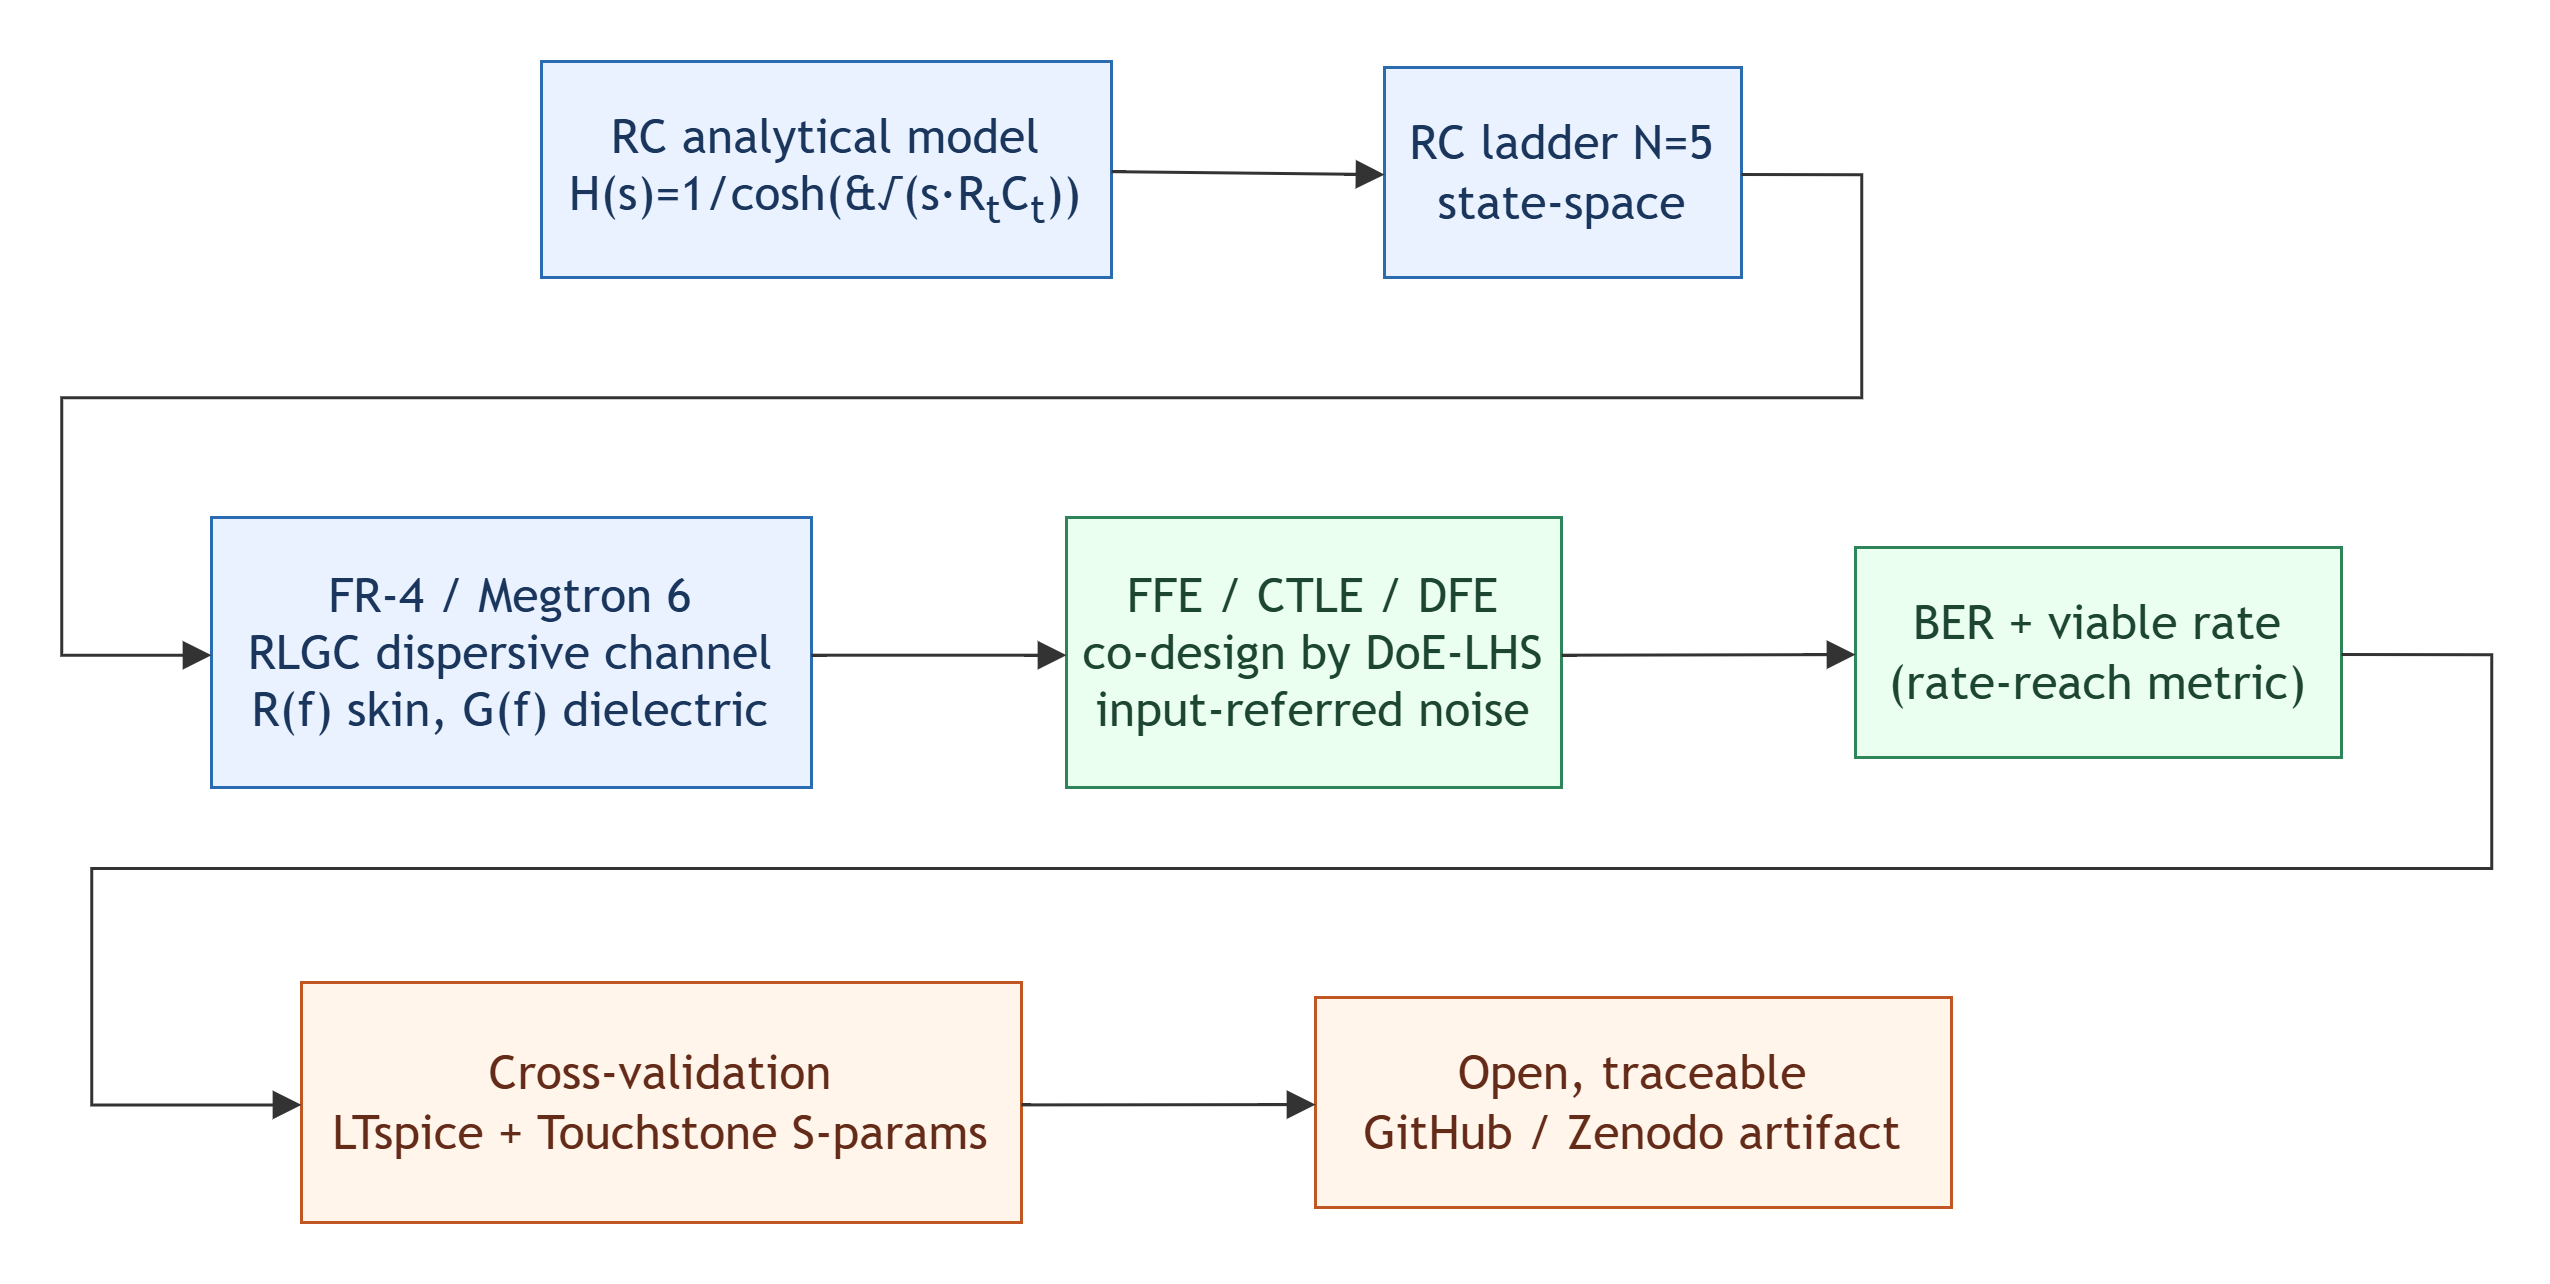
\includegraphics[width=\linewidth]{fig_flujo_conceptual.png}}{%
  \framebox[\linewidth]{\parbox[c][3cm][c]{0.88\linewidth}{\centering\footnotesize
  [Conceptual flow figure --- render \texttt{fig\_flujo\_conceptual.mmd} to
  \texttt{fig\_flujo\_conceptual.png}]}}}
\caption{Methodological flow of the reproducible transferability framework:
from the analytical RC model and the FR-4/Megtron~6 RLGC channels to
FFE/CTLE/DFE co-design, BER/rate-reach evaluation, implementation checks and
the released reproducibility artifact.}
\label{fig:flow}\end{figure}

\subsection{Distributed RC channel model}
The channel is described as a distributed-parameter RC line. Neglecting
inductance and conductance, the telegrapher's equations reduce to the
diffusion equation
\begin{equation}
\frac{\partial^2 v(x,t)}{\partial x^2} = R_0 C_0\,\frac{\partial v(x,t)}{\partial t},
\label{eq:difusion}
\end{equation}
whose transfer function, for a line of length $d$ with an open-circuit
termination, is
\begin{equation}
H(s) = \frac{1}{\cosh\!\left(\sqrt{s\,R_t C_t}\right)},
\label{eq:cosh}
\end{equation}
with $R_t=R_0 d$ and $C_t=C_0 d$. Since \eqref{eq:cosh} is transcendental, it is approximated by a ladder
network of $N$ R--C cells represented in state space
($\dot{\mathbf{v}}=\mathbf{A}\mathbf{v}+\mathbf{B}u$,
$y=\mathbf{C}\mathbf{v}$) \cite{5152908,5697500}; alternatively, a rational
Pad\'e approximation may be used \cite{554593}. The validity of the
approximation is verified by comparing its Bode plot with that of
\eqref{eq:cosh} (Section~\ref{sec:results}). The reference channel has
$R_t=80\,\Omega$ and $C_t=5\,\mathrm{pF}$ ($R_tC_t=400\,\mathrm{ps}$,
$-3\,\mathrm{dB}$ bandwidth $\approx 0.97\,\mathrm{GHz}$); the time constant
scales as $R_tC_t\propto d^2$.

\subsection{Physics-based dispersive PCB channel model}
\label{sec:canalfisico}
To overcome the diffusive idealization, a transmission line with
frequency-dependent losses is additionally considered. The per-unit-length
parameters incorporate a series resistance with skin effect and a
dielectric conductance,
\begin{equation}
\begin{aligned}
R(f)&=\sqrt{R_{dc}^2+\left(k_s\sqrt{f}\right)^2},\\
G(f)&=2\pi f\,C\,\tan\delta,
\end{aligned}
\label{eq:rlgc}
\end{equation}
so that the propagation constant
\[
\gamma(f)=\sqrt{(R+j\omega L)(G+j\omega C)}=\alpha(f)+j\beta(f)
\]
exhibits an
attenuation that grows with frequency \cite{9888577,8861405}. The model is
parameterized for two representative substrates, FR-4
($\tan\delta\approx0.020$) and Megtron~6 ($\tan\delta\approx0.004$)
\cite{9785524,10385078}, and both are compared under two criteria: the same
insertion loss as the RC channel at the Nyquist frequency of the nominal
$4\,\mathrm{GBaud}$ operating point (that is, at $2\,\mathrm{GHz}$; the
\textit{equal\_il} criterion matches the loss at that frequency and does not
imply equal severity when the swept rate exceeds the nominal point), and a
common physical length of $10$~inches (the \textit{fixed} criterion). The
channel, in its RC or dispersive form, is applied in the frequency domain
through its transfer function; the equivalence with the time-domain
simulation is verified by reproducing, through the $N=5$ ladder, the
reference result (Section~\ref{sec:results}) \cite{7445206}. As an
independent verification of the model and its implementation, the scattering
parameters of the channel are exported to Touchstone format and the chain is
additionally reproduced in a circuit simulator (LTspice), contrasting both
paths with the frequency-domain evaluation (Section~\ref{sec:results}).

Two properties of this channel class should be made explicit, because they
separate it from the wireless setting in which equalization is more commonly
discussed. First, the dispersive channel is \emph{not} realized from RC
parameters: \eqref{eq:cosh} and \eqref{eq:rlgc} are two different physical
models, and measuring the cost of substituting one for the other is precisely
the object of this work. Second, a guided copper channel exhibits neither
multipath fading nor any channel statistics to be estimated: $H(f)$ is
deterministic and time invariant, fixed by the trace geometry and the laminate,
and is therefore known by construction rather than acquired through channel
estimation. The only stochastic elements of the experiment are the data pattern
and the receiver noise. The mechanism that plays the role of multipath in a
guided line is reflection at impedance discontinuities---via stubs, connectors,
section changes---which produces delayed replicas of the pulse that are
repeatable rather than random, and are therefore addressed by layout and
equalization instead of diversity. Their effect is quantified in
Section~\ref{sec:results}.

\subsection{Test source}
The link is excited with a pseudorandom binary sequence (PRBS) generated by
a linear-feedback shift register (PRBS23, primitive polynomial) with a fixed
seed, which guarantees the reproducibility of the experiment. The sequence
presents a balance close to $50\%$ and the worst-case transitions that
stress the channel ISI. The 30 independent realizations used in the sweeps
do not change the register seed: each realization takes a \emph{disjoint
window} of the same PRBS23 sequence and a \emph{paired noise realization}
(noise seed $1000{+}r$ for realization $r$, identical across channels and
configurations so that the comparison is paired and fair). Thus, the
reported variability comes from the data pattern and the noise, not from a
change of the generator seed.

\subsection{Modulation}
Gray-coded PAM-4 signaling is used, with equispaced levels in
$\pm 3\,\mathrm{V}$ and two bits per symbol, which halves the bandwidth
requirement relative to NRZ signaling \cite{7964959}. The demonstrator
operating point is $4\,\mathrm{GBaud}$ (Nyquist frequency $2\,\mathrm{GHz}$)
with oversampling of 32 samples per symbol. As a stress case, PAM-8 is used
(eight levels within the same $\pm 3\,\mathrm{V}$ amplitude budget, with a
level spacing $\approx 2.3\times$ smaller), representative of dense
constellations in bandwidth-limited systems \cite{8963973}.

\subsection{Equalizers and receiver}
The equalization chain combines three stages, as is common in high-speed
serial links \cite{10260232,10811094}. At the transmitter, a three-tap FIR
feed-forward equalizer (FFE)
\begin{equation}
x_{\mathrm{eq}}[n] = c_{-1}\,x[n{+}1] + c_{0}\,x[n] + c_{1}\,x[n{-}1],
\label{eq:ffe}
\end{equation}
The taps are selected as relative coefficients and then scaled by the
amplitude normalization (swing constraint) $\sum_i |c_i|=1$, which bounds
the excursion of the pre-emphasized signal and must not be confused with a
power constraint ($\sum_i c_i^2$). At the receiver, a one-zero,
two-pole continuous-time linear equalizer (CTLE) \cite{10873709}
\begin{equation}
H_{\mathrm{CTLE}}(s) = A_{DC}\,\frac{1+s/\omega_z}{(1+s/\omega_{p1})(1+s/\omega_{p2})},
\label{eq:ctle}
\end{equation}
with $A_{DC}=2.5$, $\omega_{p1}=2\pi\!\cdot\!15\,\mathrm{GHz}$ and
$\omega_{p2}=2\pi\!\cdot\!30\,\mathrm{GHz}$. Finally, a decision-feedback
equalizer (DFE) cancels the ISI post-cursors,
\begin{equation}
y_{\mathrm{eq}}[n] = y[n] - \sum_{i\ge 1} b_i\,\hat{x}[n{-}i],
\label{eq:dfe}
\end{equation}
whose coefficients are estimated by least squares from the transmitted
sequence and the aligned samples (data-aided fitting), which avoids the
phase mismatch between the design pulse and the sampling instant when the
channel exhibits propagation delay \cite{11346689}. Because it is estimated
with the known transmitted sequence, the decision feedback here operates in
an aided condition (a performance bound) and not as a blind adaptive
implementation; this condition bounds the interpretation of all figures that
include it. The receiver incorporates \emph{input-referred AWGN} (injected
at the channel output, before the CTLE, with
$\sigma_{in}=0.10\,\mathrm{V}$) and a \emph{finite-bandwidth filter}
($\approx$ symbol rate). In this way the CTLE amplifies signal and noise
alike, and its benefit comes from the frequency boost, avoiding the SNR
overestimation that occurs when noise is injected after the equalizer gain
\cite{9707817}.

\emph{How the three stages act on the ISI, and how they are implemented.} The
chain is evaluated in the order TX-FFE, channel, noise injection, RX-CTLE,
receiver filter, sampling, DFE. The FFE is applied in the symbol domain as the
three-tap FIR of \eqref{eq:ffe}; the symbol stream is then oversampled to
$S=32$ samples per symbol, and both the channel and the CTLE are applied as
multiplication by their transfer functions on the discrete Fourier transform of
that sequence, which is equivalent to a zero-state time-domain simulation of
the same linear time-invariant blocks and is what makes the rate sweeps
affordable. The receiver filter is a third-order low-pass at approximately the
symbol rate, and the DFE operates on the sampled sequence as described in
Section~\ref{sec:detector}. The two variables explored by the co-design map
directly onto this chain: $\omega_z$ is the CTLE zero in \eqref{eq:ctle} and
$c_{post}$ is the post-cursor tap in \eqref{eq:ffe}.

The three stages therefore attack the same ISI from different sides, and this
is what makes their interaction the object of the study rather than an
implementation detail. The FFE pre-distorts at the transmitter, so it shapes
the pulse without amplifying receiver noise but spends transmit amplitude; the
CTLE boosts at the receiver, after the noise has been added, so it amplifies
signal and noise together; the DFE subtracts already-decided post-cursors, so
it removes ISI without any noise enhancement but cannot act on the pre-cursor.
Since the channel response is deterministic and known by construction---no
channel estimation is involved, as noted in
Section~\ref{sec:canalfisico}---the design question is not how to acquire the
channel but how to distribute the compensation among three stages whose costs
differ, which is what Sections~\ref{sec:results} onward measure.

\subsection{Symbol detection at the receiver}
\label{sec:detector}
The detector operates on one sample per symbol and is fully deterministic; it
is specified here in full because every reported error rate is produced by it.

\emph{Sampling instant.} The receiver takes one sample per symbol at the phase
$\varphi\in\{0,\dots,S-1\}$ ($S=32$ samples per symbol) and integer symbol
delay $\ell$ that maximize the normalized correlation between the subsampled
stream $y[\varphi+kS]$ and the transmitted symbols $a_k$,
\begin{equation}
(\varphi^{\ast},\ell^{\ast})=\arg\max_{\varphi,\ell}
\frac{\left|\sum_{k}\tilde{y}[\varphi+(k{+}\ell)S]\,\tilde{a}_k\right|}
{\|\tilde{y}\|\,\|\tilde{a}\|},
\label{eq:fase}
\end{equation}
where $\tilde{(\cdot)}$ denotes the mean-removed sequence. This is a
data-aided timing recovery: like the DFE fitting, it is a performance bound
rather than a blind loop, and it prevents sampling at the eye crossing. The
first $100$ symbols are discarded as the chain transient. Fig.~\ref{fig:detector}(a)
shows that the choice is not cosmetic: on the FR-4 channel at the operating
point the correlation falls from $0.995$ at $\varphi^{\ast}=0.625$~UI to
$0.723$ at the worst phase.

\emph{Decision feedback.} With an $n$-tap DFE, the corrected sample is
$y_k=m_k-\sum_{i=1}^{n} h_i\,\hat{a}_{k-i}$, where $m_k$ is the sample from
\eqref{eq:fase}, the coefficients $h_i$ are the least-squares fit of
\eqref{eq:dfe} on the aligned samples, and $\hat{a}_{k-i}$ is the previous hard
decision, taken as the nearest PAM-4 level scaled by the fitted cursor gain
$h_0$.

\emph{Thresholds and error rate.} Let $\mu_k$ and $\sigma_k$ be the mean and
standard deviation of the samples whose transmitted symbol is level $k$, both
estimated from the received signal, so that $\sigma_k$ aggregates residual ISI
and noise. The decision thresholds are the midpoints between adjacent received
means,
\begin{equation}
\tau_k=\frac{\mu_k+\mu_{k+1}}{2},\qquad k=1,2,3,
\label{eq:umbral}
\end{equation}
that is, they adapt to the received levels rather than being fixed at the
nominal ones. The error probability of each level follows from the Gaussian
tails that cross its thresholds---one tail for the outer levels, two for the
inner ones,
\begin{equation}
P_{e,k}=Q\!\left(\frac{|\tau_{k}-\mu_k|}{\sigma_k}\right)
+Q\!\left(\frac{|\mu_k-\tau_{k-1}|}{\sigma_k}\right),
\label{eq:pek}
\end{equation}
with the convention that terms involving a nonexistent threshold are omitted.
Weighting by the observed frequency $p_k$ of each level gives the symbol error
rate, and Gray coding maps a decision error between adjacent levels to a single
wrong bit out of the two carried by the symbol, so that
\begin{equation}
\mathrm{SER}=\sum_{k=1}^{4}p_k\,P_{e,k},
\qquad
\mathrm{BER}=\frac{\mathrm{SER}}{2}.
\label{eq:ber}
\end{equation}
The worst-eye opening reported in Section~\ref{sec:results} is obtained from
the same statistics as
$\min_k\left[(\mu_{k+1}-3\sigma_{k+1})-(\mu_k+3\sigma_k)\right]$.
Fig.~\ref{fig:detector}(b)--(c) shows the resulting level distributions and
thresholds with and without decision feedback: the feedback stage does not
displace the levels but narrows each of them, which is what lowers the BER from
$8.0\times10^{-6}$ to $6.8\times10^{-7}$ at the operating point.

\begin{figure*}[!t]\centering
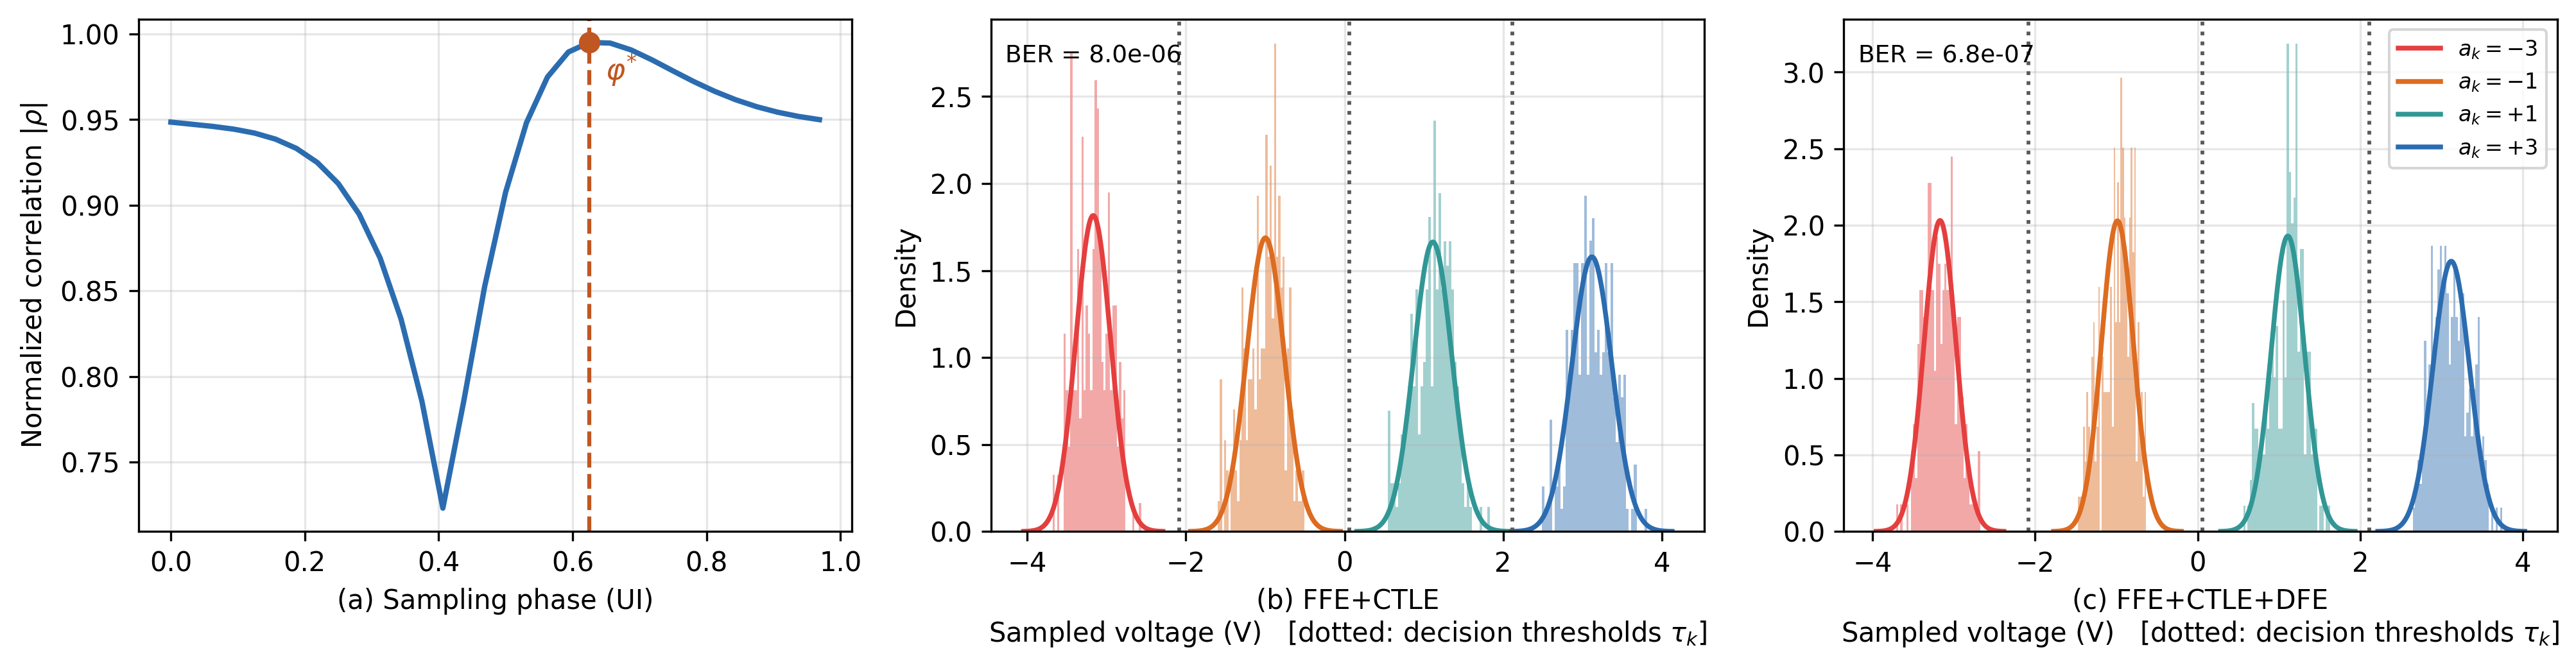
\includegraphics[width=\textwidth]{fig_detector_niveles.png}
\caption{Symbol detection on the FR-4 channel at the 4~GBaud operating point:
(a)~selection of the sampling instant by normalized correlation, (b)~sampled
level distributions, Gaussian fits and decision thresholds $\tau_k$ after
FFE+CTLE, and (c)~the same after adding the two-tap decision-feedback stage.}
\label{fig:detector}\end{figure*}

\subsection{Co-design by design of experiments}
Since the number of equalization combinations grows with the rate, the
co-design space is explored with design of experiments (DoE) rather than
exhaustive search \cite{7851249,5770781}. Latin hypercube sampling is
applied over the two variables that dominate the eye opening---the CTLE zero
$\omega_z$ and the FFE post-cursor $c_{post}$---with 30 samples; the
objective is the actual vertical opening of the worst eye ($3\sigma$ margin
to ISI). The selected point is fixed for the subsequent simulations. For the
dispersive channels, since the optimal tuning depends on the channel loss
profile, the co-design is re-optimized per substrate on the dispersive channel model
\cite{11169790}. The optimization can be performed in stages---taking the
linear-equalizer eye opening as the objective---or jointly over the full
chain---taking the viable rate with decision feedback as the objective and
incorporating the CTLE gain $A_{DC}$ into the design space---to prevent an
excessive linear boost from penalizing the feedback stage. The framework
admits extension to sequential or Bayesian-optimization schemes
\cite{11309336}.

\subsection{Evaluation variables and indicators}
The evaluation is structured on the operationalization of two variables. The
\emph{independent variable} is the co-designed equalization strategy, whose
dimensions are the TX-FFE, RX-CTLE and RX-DFE stages
(\eqref{eq:ffe}--\eqref{eq:dfe}) and the DoE tuning described above. The
\emph{dependent variable} is the link performance, measured by four
end-point indicators:

\begin{itemize}
\item \textbf{Rate reach} (primary indicator): viable symbol rate, defined
as the interpolated crossing---on a $\log_{10}(\mathrm{BER})$ scale---of the
pre-FEC threshold ($\mathrm{BER}\le 10^{-2}$) in a rate sweep; its value is
reported as mean $\pm$ standard deviation over 30 independent PRBS-pattern
and noise realizations. The $10^{-2}$ threshold is compatible with a strong
forward error correction (FEC) of the KP4/RS family common in high-speed
links; since it depends on the assumed FEC scheme and is not universal, it
is complemented by a sensitivity analysis to stricter thresholds ($10^{-3}$
and $10^{-4}$, Section~\ref{sec:results}).
\item \textbf{Signal integrity (vertical margin)}: worst-eye opening,
measured as the $3\sigma$ margin between adjacent PAM levels at the optimal
sampling instant.
\item \textbf{Timing margin (horizontal margin)}: horizontal eye opening,
obtained from the error-rate curve versus the sampling phase, injecting
random (Gaussian) and deterministic (dual-Dirac worst-case, or sinusoidal
periodic) jitter at the receiver sampling instant \cite{805809,9874925}. The
horizontal opening is obtained by equal-error-rate interpolation on the
bathtub curve, in line with BER-based eye reconstruction methods
\cite{Chen2024BER}.
\item \textbf{Reliability}: \emph{semi-analytical} BER, obtained from the
detector of Section~\ref{sec:detector} through
\eqref{eq:umbral}--\eqref{eq:ber}, which avoids the prohibitive cost of Monte
Carlo counting of low BERs \cite{6248821,7202856,10415105}. This estimate assumes Gaussian
tails per level, an assumption that conditions the interpretation of all BER
and viable-rate results and that is contrasted against Monte Carlo counting
in the feasible region (Section~\ref{sec:results}). Estimates below
$10^{-12}$ are reported as \emph{below the reporting floor} (extrapolated
BER $<10^{-12}$), since in that region the Gaussian tail is no longer
reliable.
\end{itemize}

This procedure is consistent with the statistical-eye and peak-distortion
analysis approaches used to evaluate high-speed links with equalization
\cite{10705630}. Table~\ref{tab:params} summarizes the complete set of
test-bench parameters, so that the result tables are reproducible from a
single recipe.

%% Master table of simulation parameters (reproducibility).
\begin{table*}[!t]
\caption{Complete set of test-bench parameters (reproducibility).}
\label{tab:params}
\centering
\footnotesize
\begin{tabular}{p{0.20\textwidth} p{0.36\textwidth} p{0.36\textwidth}}
\hline
\textbf{Group} & \textbf{Parameter} & \textbf{Value} \\
\hline
\multirow{3}{*}{RC channel}
 & Total resistance/capacitance; time constant & $R_t=80\,\Omega$, $C_t=5\,\mathrm{pF}$, $\tau=R_tC_t=400\,\mathrm{ps}$ \\
 & Ladder approximation; $-3$~dB bandwidth & $N=5$ R--C cells (state space); $\approx0.97\,\mathrm{GHz}$ \\
 & Analytical reference transfer function & $H(s)=1/\cosh(\sqrt{s\,R_tC_t})$ \\
\hline
\multirow{5}{*}{Physical lines (RLGC)}
 & Microstrip geometry (common) & $Z_0=50\,\Omega$, width $w=150\,\mu\mathrm{m}$, thickness $t=35\,\mu\mathrm{m}$ (1~oz) \\
 & FR-4 / Megtron~6 substrate & $D_k=4.3$, $\tan\delta=0.020$ / $D_k=3.6$, $\tan\delta=0.004$ \\
 & $f$-dependent losses & $R(f)=\sqrt{R_{dc}^2+(k_s\sqrt{f})^2}$, $k_s=\sqrt{\pi\mu_0/\sigma}/w$; $G(f)=2\pi f C\tan\delta$ \\
 & Lengths (\textit{equal\_il} criterion) & FR-4 $22.9''$, Megtron~6 $36.9''$ (match RC IL${=}7.38\,\mathrm{dB}$ at $2\,\mathrm{GHz}$) \\
 & Length (\textit{fixed} criterion) & $10''$ both \\
\hline
\multirow{4}{*}{Source and sampling}
 & Pattern; polynomial & PRBS23, feedback on taps $[23,18]$, fixed seed \\
 & Symbols per realization; oversampling & $N_{\mathrm{sym}}=1000$; $\mathrm{sps}=32$ ($F_s=32\,R_s$) \\
 & Realizations; scheme & $30$; disjoint PRBS window per realization + paired noise \\
 & Noise seed (realization $r$) & $1000+r$ (identical across channels/configurations) \\
\hline
\multirow{2}{*}{Receiver}
 & Input-referred AWGN (pre-CTLE) & $\sigma_{in}=0.10\,\mathrm{V}$ \\
 & Finite-bandwidth filter & 3rd-order Butterworth, $f_c=R_s$ \\
\hline
\multirow{3}{*}{Equalization}
 & FFE (3 taps) $[c_{pre},c_{main},c_{post}]$; normalization & relative $[0,\,1,\,-0.301]$; scaled to amplitude $\sum_i|c_i|=1$ \\
 & CTLE (1 zero, 2 poles) & $A_{DC}=2.5$, $\omega_z=2\pi\!\cdot\!2.35\,\mathrm{GHz}$, $\omega_{p1}=2\pi\!\cdot\!15$, $\omega_{p2}=2\pi\!\cdot\!30\,\mathrm{GHz}$ \\
 & DFE & 2 post-cursors; data-aided (least squares on aligned samples) \\
\hline
\multirow{2}{*}{Alignment / DoE}
 & Sampling-phase selection & coarse delay by FFT + optimal phase $0..\mathrm{sps}{-}1$ by correlation \\
 & DoE-LHS: ranges / samples / seeds & $\omega_z\!\in\![1,10]\,\mathrm{GHz}$, $c_{post}\!\in\![-0.40,-0.05]$, $A_{DC}\!\in\![1,3]$; $30$ (re-DoE) / $24$ (joint); seeds $42$ / $11$ \\
\hline
\multirow{2}{*}{BER metric}
 & Viability threshold; interpolation; floor & pre-FEC $\mathrm{BER}\le10^{-2}$; linear in $\log_{10}(\mathrm{BER})$; report $10^{-12}$ \\
 & Estimator & semi-analytical ($Q$ function, per-level Gaussian assumption) \\
\hline
\end{tabular}
\end{table*}


%% =====================================================================
\section{Results}
\label{sec:results}

The common conditions are: PRBS23 source, PAM-4 modulation, receiver
input-referred noise ($\sigma_{in}=0.10\,\mathrm{V}$) and finite receiver
bandwidth (approximately the symbol rate). The BER is estimated by the
semi-analytical method with a reporting floor of $10^{-12}$. The viable rate
is interpolated at the crossing of the pre-FEC threshold
($\mathrm{BER}\le10^{-2}$) and reported as mean $\pm$ standard deviation over
30 pattern and noise realizations. Unless stated otherwise, the co-design is
the one inherited from the RC channel
($\omega_z=2\pi\cdot2.35\,\mathrm{GHz}$, $c_{post}=-0.301$; one-zero,
two-pole CTLE, $A_{DC}=2.5$; two-tap DFE). Four channels are contrasted: the
distributed RC ($1/\cosh$ and its order-$N=5$ ladder), and two physical
transmission lines with frequency-dependent losses (FR-4 and Megtron~6
substrates), under two comparison criteria: equal insertion loss at Nyquist
(\textit{equal\_il}) and fixed physical length of 10~inches (\textit{fixed}).

\subsection{Model validation and physical-channel characterization}
The ladder approximation reproduces the analytical response for $N\ge5$
cells up to the GHz range; lower orders diverge beyond approximately 1~GHz
(Fig.~\ref{fig:bode}). The $-3$~dB bandwidth of the reference channel is
0.97~GHz. As a quantitative validation of the simulator, the rate sweep over
the $N=5$ ladder reproduces the reference result within 3--5\,\%: $2.88$,
$9.76$ and $13.73$~GBaud for no equalization, FFE+CTLE and FFE+CTLE+DFE,
against $2.79$, $9.56$ and $14.11$~GBaud for the reference. The exact
$1/\cosh$ model is somewhat more optimistic (up to $15.21$ and
$19.38$~GBaud), since the low-order ladder is conservative in the band that
equalization exploits.

\begin{figure}[!t]\centering

\includegraphics[width=\linewidth]{fig_bode.png}
\caption{Frequency response of the order-$N$ ladder approximation against the
analytical solution $1/\cosh(\sqrt{j\omega R_tC_t})$.}
\label{fig:bode}\end{figure}

Replacing the RC line with a transmission-line model with skin effect $R(f)$
and dielectric loss $G(f)$, the channel changes from diffusive to dispersive
behavior. The attenuation grows with frequency (Fig.~\ref{fig:aten}): at
Nyquist (2~GHz) it is approximately $0.32$~dB/inch for FR-4 and
$0.20$~dB/inch for Megtron~6 (loss tangents $0.020$ and $0.004$), with a
separation that widens at high frequency. The pulse response
(Fig.~\ref{fig:pulso}), matched to the same RC loss at Nyquist (7.4~dB;
equivalent lengths of 22.9 and 36.9~inches), reveals a real propagation
delay ($\approx$3--5~ns) absent in the lumped RC model, and a distinct ISI
tail.

\begin{figure}[!t]\centering

\includegraphics[width=\linewidth]{fig_atenuacion_dbporpulgada.png}
\caption{Attenuation in dB/inch versus frequency for FR-4 and Megtron~6
(skin effect plus dielectric loss).}
\label{fig:aten}\end{figure}

\begin{figure}[!t]\centering

\includegraphics[width=\linewidth]{fig_respuesta_pulso.png}
\caption{Pulse response: diffusive RC channel against the dispersive FR-4 and
Megtron~6 lines, matched to the same insertion loss at Nyquist.}
\label{fig:pulso}\end{figure}

As a numerical cross-check of the model, its scattering parameters
($S$-parameters) were exported to Touchstone format referenced to
$50\,\Omega$. The network is passive across the whole band
($|S_{11}|^2+|S_{21}|^2\le0.97$) and its $S_{21}$ matches the transfer
function used in the chain within $0.01$~dB up to $4$~GHz, with discrepancies
attributable to reflections from the deviation of $Z_c$ from $50\,\Omega$;
the Touchstone files also serve as a bridge to commercial tools (SPICE/ADS).
Likewise, a sensitivity analysis (Fig.~\ref{fig:senscanal}) shows that the
viable rate depends smoothly on the loss tangent (from $16.8$ to
$13.7$~GBaud as $\tan\delta$ varies from $0.002$ to $0.025$), strongly on the
length (from $15.1$ to $6.4$~GBaud between $5$ and $32$~inches) and only
marginally on the surface roughness (Hammerstad correction: $<0.6$~GBaud up
to $1\,\mu\mathrm{m}$ RMS), which identifies the dielectric loss and the
length as the dominant factors and the roughness as a second-order effect in
this range.

\begin{figure}[!t]\centering

\includegraphics[width=\linewidth]{fig_sensibilidad_canal.png}
\caption{Sensitivity of the viable rate (FFE+CTLE, inherited EQ) to the loss
tangent, the length and the surface roughness of the dispersive channel.}
\label{fig:senscanal}\end{figure}


As an additional cross-check, the chain was reproduced in an independent
circuit simulator (LTspice). The five-cell RC ladder, the CTLE---as a
transfer function---and the FFE---as a delay line---map directly to circuit
elements, while the dispersive lines are incorporated through a stable
rational fit of their $S$-parameters. In the frequency domain, the response
of the RC channel and the CTLE in the circuit simulator matches the transfer
function used in the chain within numerical error, and the dispersive line
reproduces its $S_{21}$ within $0.6$~dB up to $15$~GHz. In the time domain,
exciting with the same PRBS23/PAM-4 sequence and the same noise realization,
the eye diagram at $4$~GBaud over the RC channel obtained with the circuit
simulator matches that of the chain evaluated in frequency
(Fig.~\ref{fig:ltspice}): the difference in worst-eye opening is below
$0.5\%$ and the sampled levels agree within $0.01$~V. The transient eye of
the dispersive lines is not addressed in the circuit simulator---the
skin-effect attenuation ($\propto\sqrt{f}$) does not admit a compact rational
representation and the dielectric loss requires the imaginary unit in the
transfer function---and is therefore obtained in the frequency-domain
processing. The agreement between two independent simulation engines
supports the implementation of the chain.

\begin{figure*}[!t]\centering

\includegraphics[width=\textwidth]{fig_ltspice_ojos.png}
\caption{PAM-4 eye diagram at 4~GBaud over the RC channel: (a)~chain
evaluated in the frequency domain, (b)~the same chain in a circuit simulator
(LTspice) excited with identical sequence and noise, and (c)~overlay of
both.}
\label{fig:ltspice}\end{figure*}

This cross-check is carried to the quantities the results are actually built
from. No hardware implementation is involved anywhere in this work: every
figure is produced by the frequency-domain chain, and the circuit simulator
provides an independent \emph{software} implementation against which that chain
is verified. Applying the detector of Section~\ref{sec:detector} to the two
engines over the same $400$-symbol sequence yields the constellations of
Fig.~\ref{fig:constelacion}, which agree sample by sample with a Pearson
coefficient of $0.99999$ and an RMS difference of $17$~mV, that is $0.41\%$ of
full scale. The per-level means agree within $17$~mV and the per-level standard
deviations within $6$~mV, so the decision thresholds \eqref{eq:umbral} derived
by each engine differ by at most $12$~mV; both give a BER below the $10^{-12}$
reporting floor for this configuration, and the worst-eye openings differ by
$30$~mV ($1.3\%$). The constellation and the error rate are therefore
properties of the modeled link and not of the tool that renders them.

\begin{figure}[!t]\centering
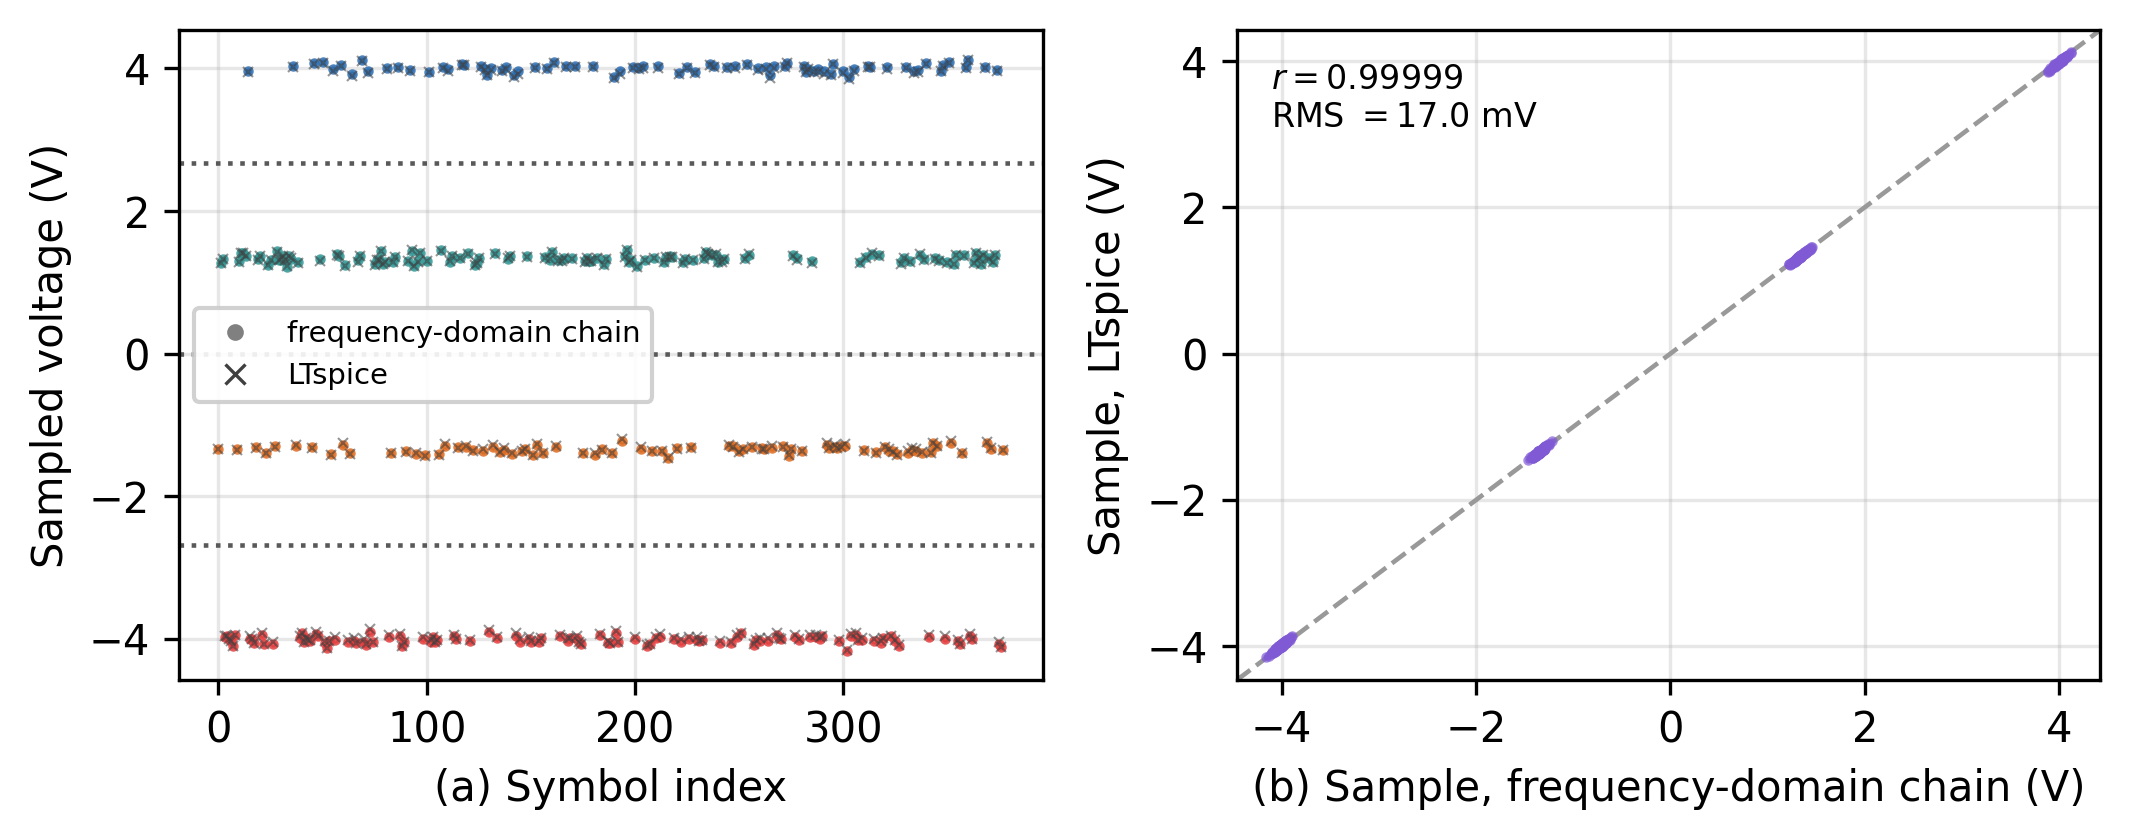
\includegraphics[width=\linewidth]{fig_constelacion_motores.png}
\caption{Cross-engine agreement at the level of the detected symbols
(RC channel, 4~GBaud, same sequence and noise realization):
(a)~PAM-4 constellation with the decision thresholds, from the frequency-domain
chain (dots) and from the circuit simulator (crosses), and (b)~sample-by-sample
correlation between the two engines.}
\label{fig:constelacion}\end{figure}

\subsection{Impedance discontinuities: the reflective analogue of multipath}
\label{sec:reflexiones}
The channels above are uniform lines. A physical board also carries impedance
discontinuities, which return delayed replicas of the pulse and are the guided
counterpart of multipath---deterministic replicas rather than random fading.
To bound their effect, the $10$-inch FR-4 trace was rebuilt as a cascade of
$ABCD$ matrices terminated in $50\,\Omega$, with a discontinuity at midpoint:
either an open-circuited via stub of length $L_s$, whose input impedance
$Z_c\coth(\gamma L_s)$ places a quarter-wave resonance at $f_{res}=v_p/(4L_s)$,
or a $0.5$-inch $35\,\Omega$ section representing a connector or pad region.
Removing the discontinuity, the cascade reproduces the matched channel
$e^{-\gamma\ell}$ used throughout this work within $10^{-4}$~dB up to
$20\,\mathrm{GHz}$, and its viable rate ($14.05\pm0.21$ and $27.27\pm0.42$~GBaud
for FFE+CTLE and FFE+CTLE+DFE) matches Table~\ref{tab:r1}, so the two models are
directly comparable.

Fig.~\ref{fig:reflexiones}(a) shows the replicas that the discontinuity adds:
the mismatched section returns a double-reflection echo at twice its transit
delay ($2\tau_d\approx138$~ps), and the stub adds resonant ringing.
Fig.~\ref{fig:reflexiones}(b) shows the corresponding spectral signature, a
notch of more than $20$~dB at $f_{res}$. The cost in viable rate
(Fig.~\ref{fig:reflexiones}(c)) is strongly asymmetric between equalization
stages: a $90$-mil stub costs the linear chain only $3.4\%$ but the full chain
$18.2\%$, and a $120$-mil stub costs $10.3\%$ and $30.7\%$. The reason is that
the penalty appears when the operating Nyquist frequency reaches the resonance:
the FFE+CTLE chain runs near $14$~GBaud, that is $7$~GHz, well below the
$15.8$~GHz notch of the $90$-mil stub, whereas the decision-feedback chain runs
near $27$~GBaud and samples exactly the notch. This yields a companion to the
design rule of Section~\ref{sec:results}: a spectral null is neither boosted
away by a linear stage nor cancelled by decision feedback, so the stub length
must satisfy $f_{res}=v_p/(4L_s)$ comfortably above the Nyquist frequency the
equalized link is expected to reach---a constraint that becomes binding
precisely because equalization extends that reach.

The mismatched section illustrates that a discontinuity is not a penalty by
construction. At $11$~GBaud it \emph{raises} the FFE+CTLE viable rate by
$6.3\%$: its echo reduces the per-level standard deviation by $21\%$ while
shrinking the level separation by only $3.4\%$, and since the receiver noise is
processed identically in both cases, that reduction is residual ISI rather than
noise---the reflected replica partially cancels the channel tail at rates where
it lands with opposite sign. The benefit is rate specific and does not survive:
with decision feedback, which operates near $26$~GBaud, the same section costs
$5.1\%$. Discontinuities must therefore be evaluated at the rate the link
actually runs, not judged from the return loss alone.

\begin{figure*}[!t]\centering
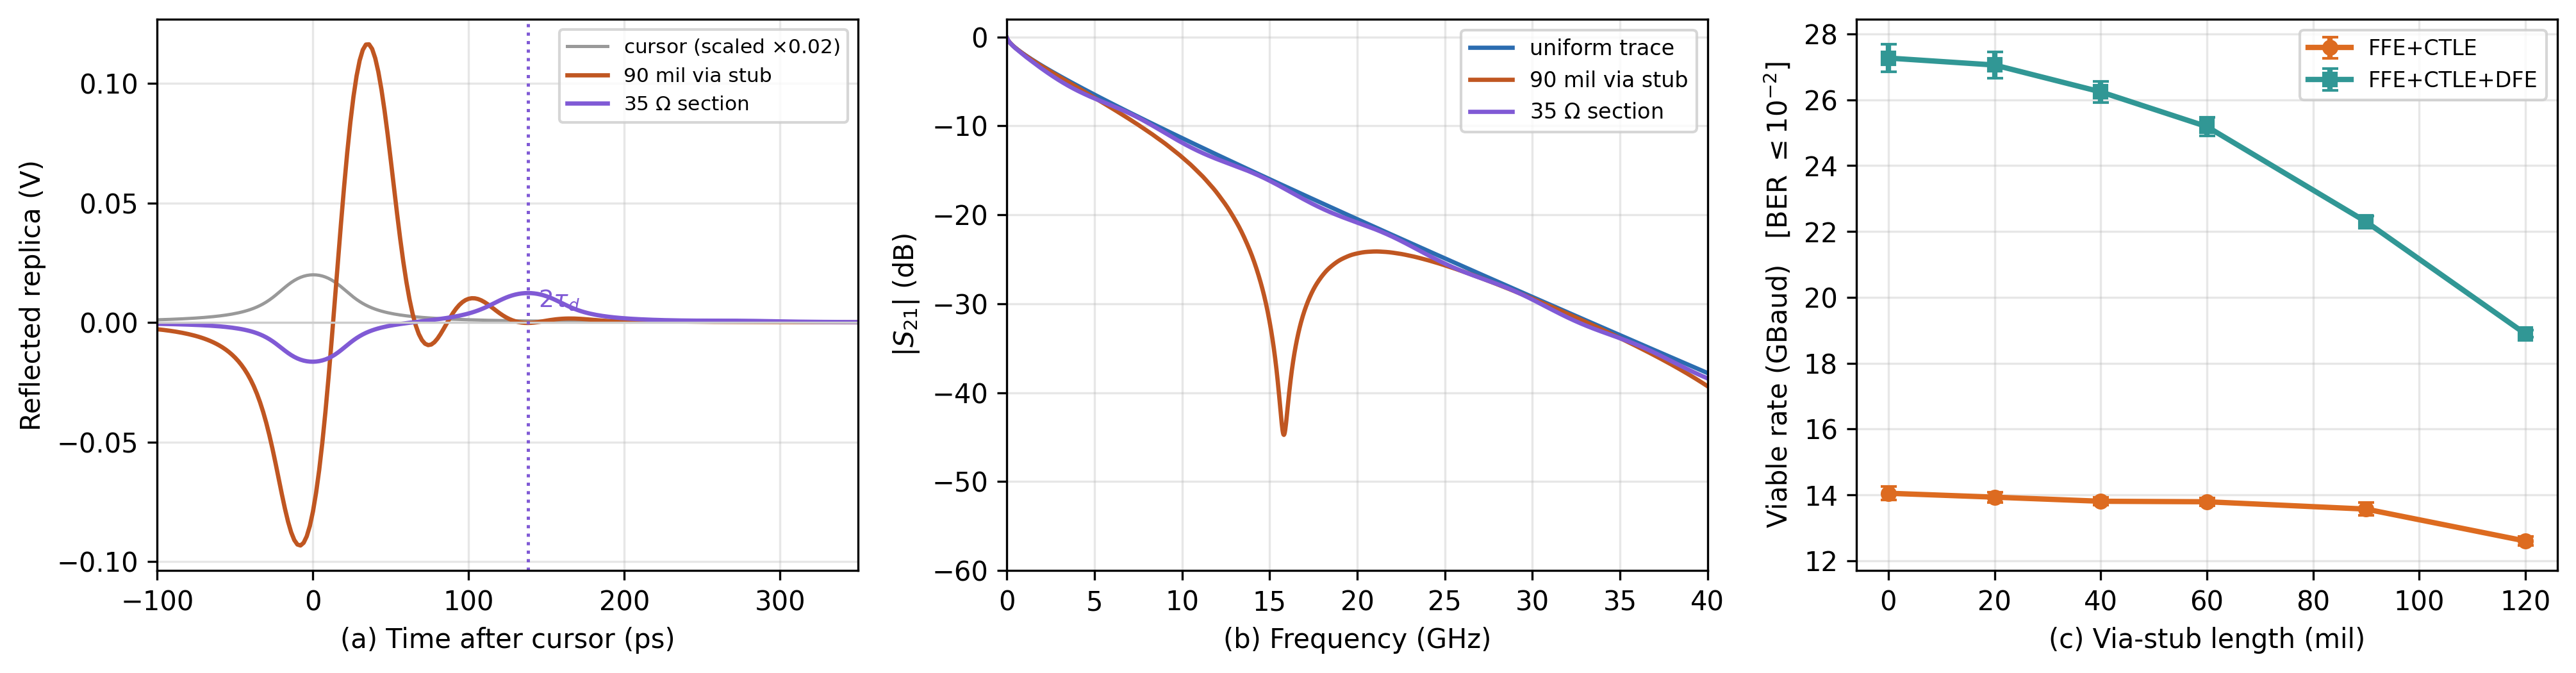
\includegraphics[width=\textwidth]{fig_reflexiones.png}
\caption{Impedance discontinuities on the 10-inch FR-4 trace: (a)~delayed
replicas added by a $90$-mil via stub and by a $0.5$-inch $35\,\Omega$ section,
plotted as the difference from the uniform trace, (b)~the resulting $|S_{21}|$
with the quarter-wave notch at $15.8$~GHz, and (c)~viable rate versus via-stub
length for the linear and the full equalization chains.}
\label{fig:reflexiones}\end{figure*}

\subsection{Viable symbol rate per configuration and channel (rate reach)}
Table~\ref{tab:r1} reports the viable rate per channel and configuration for
the two criteria, and Fig.~\ref{fig:ratesweep} shows the BER sweeps. At
equal loss at Nyquist (\textit{equal\_il}), \emph{without equalization the
dispersive channels tolerate a higher rate than the RC} (4.6 and 5.2 versus
2.9~GBaud): the diffusive RC channel is the most pessimistic because of its
prolonged ISI tail. Under fixed physical length (\textit{fixed}), the real
10-inch traces are very capable (FFE+CTLE+DFE reaches 27.2~GBaud on FR-4 and
exceeds 60~GBaud on Megtron~6 after extending the sweep). On Megtron~6
\textit{fixed}, \emph{over-equalization} is observed: FFE+CTLE reduces the
viable rate (16.3 versus 40.1~GBaud unequalized) because the CTLE amplifies
noise unnecessarily over an almost lossless channel.

\begin{table}[!t]
\caption{Viable Symbol Rate (GBaud, Mean $\pm$ Standard Deviation, 30
Realizations; $\mathrm{BER}\le10^{-2}$). EQ Inherited From the RC.}
\label{tab:r1}\centering
\begin{tabular}{llccc}
\hline
\textbf{Crit.} & \textbf{Channel} & \textbf{No EQ} & \textbf{FFE+CTLE} & \textbf{+DFE} \\
\hline
\textit{eq\_il} & RC ($N{=}5$)   & $2.88{\pm}0.01$ & $9.76{\pm}0.18$ & $13.73{\pm}0.29$ \\
\textit{eq\_il} & FR-4 (22.9'')  & $4.58{\pm}0.11$ & $9.31{\pm}0.23$ & $9.71{\pm}0.23$ \\
\textit{eq\_il} & Megtron (36.9'')& $5.16{\pm}0.21$ & $10.83{\pm}0.28$ & $11.88{\pm}0.41$ \\
\hline
\textit{fixed}  & FR-4 (10'')    & $12.75{\pm}0.28$ & $14.06{\pm}0.31$ & $27.19{\pm}0.49$ \\
\textit{fixed}  & Megtron (10'') & $40.1{\pm}1.3$ & $16.27{\pm}0.15$ & $\ge 64^{\ast}$ \\
\hline
\end{tabular}
\par\smallskip
\footnotesize{$^{\ast}$ The sweep was extended to 64~GBaud to resolve the
saturations; the FFE+CTLE+DFE case on Megtron~6 still does not cross the
$10^{-2}$ threshold within the sweep and is reported as a lower bound (at a
$10^{-4}$ threshold the viable rate is finite, $\approx56$~GBaud;
Table~\ref{tab:rumbral}).}
\end{table}

\begin{figure*}[!t]\centering

\includegraphics[width=0.49\textwidth]{fig_barrido_tasa_equal_il.png}\hfill

\includegraphics[width=0.49\textwidth]{fig_barrido_tasa_fixed.png}
\caption{Semi-analytical BER versus PAM-4 symbol rate (median and envelope
over 30 realizations) for no equalization, FFE+CTLE and FFE+CTLE+DFE. Left:
equal-loss-at-Nyquist criterion; right: fixed physical length of 10~inches.}
\label{fig:ratesweep}\end{figure*}

\subsection{Signal integrity: eye diagram}
Fig.~\ref{fig:ojos} shows the PAM-4 eye diagrams at the operating point
(4~GBaud) over the dispersive channel model: without equalization the eye is closed,
and the co-design chain progressively recovers it (FFE, FFE+CTLE) until the
DFE tightens the decision levels. Table~\ref{tab:r2} quantifies the
worst-eye opening per scenario and channel: it is negative without
equalization (closed eye) and positive at all equalized stages. The RC
channel reaches a larger opening after the CTLE than the dispersive channels
(a more modest opening despite the same boost), which anticipates that the
inherited co-design is not adapted to the dispersive channel model
(Table~\ref{tab:r4}).

\begin{table}[!t]
\caption{Worst-Eye Opening (V) at the Operating Point (4~GBaud, Equal-Loss Physical-Channel Criterion).}
\label{tab:r2}\centering
\begin{tabular}{lcccc}
\hline
\textbf{Channel} & \textbf{No EQ} & \textbf{FFE} & \textbf{FFE+CTLE} & \textbf{+DFE} \\
\hline
RC ($N{=}5$) & $-1.78$ & $+0.51$ & $+2.14$ & $+2.19$ \\
FR-4         & $-0.29$ & $+0.30$ & $+0.66$ & $+0.83$ \\
Megtron 6    & $-0.16$ & $+0.28$ & $+0.60$ & $+0.65$ \\
\hline
\end{tabular}
\end{table}

\begin{figure*}[!t]\centering
\includegraphics[width=\textwidth]{fig_ojo_escenarios.png}
\caption{PAM-4 eye diagrams at 4~GBaud (FR-4 channel): A (no equalization), B
(FFE), C (FFE+CTLE) and sampled levels with and without DFE.}
\label{fig:ojos}\end{figure*}

\subsection{Reliability: BER at the operating point}
The reliability behavior is consistent with the viable rate
(Table~\ref{tab:r1}): at 4~GBaud, without equalization the RC channel is not
viable (BER $7.4\times10^{-2}$, above the threshold, since its limit rate of
2.9~GBaud lies below the operating point), whereas the dispersive channels
are viable ($4.6\times10^{-3}$ and $2.4\times10^{-3}$). All equalized
configurations operate below the pre-FEC threshold (Table~\ref{tab:r3}).
Note that the equalized RC reaches $<10^{-12}$ while the dispersive channels
remain around $10^{-6}$: the equalization inherited from the RC, although
sufficient, is not adapted to the dispersive channel model, which motivates the
re-co-design (Table~\ref{tab:r4}).

\begin{table}[!t]
\caption{Semi-Analytical BER per Scenario and Channel (4~GBaud, Equal-Loss Physical-Channel Criterion).}
\label{tab:r3}\centering
\begin{tabular}{lcccc}
\hline
\textbf{Channel} & \textbf{No EQ} & \textbf{FFE} & \textbf{FFE+CTLE} & \textbf{+DFE} \\
\hline
RC ($N{=}5$) & $7.4{\times}10^{-2}$ & $1.6{\times}10^{-10}$ & $<10^{-12}$ & $<10^{-12}$ \\
FR-4         & $4.6{\times}10^{-3}$ & $1.3{\times}10^{-6}$ & $4.9{\times}10^{-6}$ & $3.4{\times}10^{-7}$ \\
Megtron 6    & $2.4{\times}10^{-3}$ & $1.8{\times}10^{-6}$ & $4.5{\times}10^{-6}$ & $2.6{\times}10^{-6}$ \\
\hline
\end{tabular}
\end{table}

\subsection{BER-estimator validation and threshold sensitivity}
To rule out that the semi-analytical estimator overestimates performance, it
was contrasted against direct Monte Carlo counting over long sequences
($\approx5\times10^{5}$ symbols per point), using the same decision
thresholds (Fig.~\ref{fig:bermc}). In the region near the pre-FEC threshold
both estimates agree---for example, FR-4 with FFE+CTLE yields
$2.4\times10^{-2}$ (semi-analytical) versus $2.3\times10^{-2}$ (Monte Carlo)
at $16$~GBaud---; below the threshold the estimator is \emph{slightly
conservative} (it predicts more errors than the counting), also with the
decision feedback in the loop. Consequently, the reported viable rates are
not optimistic: the Gaussian assumption does not inflate performance in the
region that defines viability.

\begin{figure}[!t]\centering

\includegraphics[width=\linewidth]{fig_validacion_ber_mc.png}
\caption{Validation of the semi-analytical BER (lines) against Monte Carlo
counting (markers) for FR-4 and Megtron~6, FFE+CTLE and FFE+CTLE+DFE
scenarios.}
\label{fig:bermc}\end{figure}

The sequence length per realization ($1000$ symbols, $\approx250$ per PAM-4
level) is sufficient because the semi-analytical estimator relies on the
per-level means and standard deviations---which converge with the number of
samples per level---and not on counting rare errors, and because the viable
rate is averaged over 30 realizations (effectively $\sim\!7500$ symbols per
level). A convergence study confirms this: when increasing the length from
$1000$ to $16000$ symbols, the viable rate varies by less than $0.3\%$ (FR-4
FFE+CTLE $13.78\!\rightarrow\!13.74$; FR-4 +DFE
$27.12\!\rightarrow\!27.11$; Megtron~6 FFE+CTLE
$16.73\!\rightarrow\!16.77$~GBaud) and the per-level standard deviations
remain within $5\%$, so that the eye means and standard deviations are
converged at the operating point.

The definition of viability depends on the assumed pre-FEC threshold.
Table~\ref{tab:rumbral} reports the viable rate of the full chain at three
thresholds ($10^{-2}$, $10^{-3}$, $10^{-4}$): although the absolute value
decreases as a stricter threshold is required, the \emph{ordering} between
channels and the relative advantage of equalization are preserved, so that
the conclusions do not depend critically on the chosen threshold.

\begin{table}[!t]
\caption{FFE+CTLE+DFE Viable Rate (GBaud, Mean $\pm$ Standard Deviation, 30
Realizations) at Different Pre-FEC Thresholds.}
\label{tab:rumbral}\centering
\begin{tabular}{llccc}
\hline
\textbf{Crit.} & \textbf{Channel} & $\mathbf{10^{-2}}$ & $\mathbf{10^{-3}}$ & $\mathbf{10^{-4}}$ \\
\hline
\textit{eq\_il} & RC ($N{=}5$)   & $13.7{\pm}0.3$ & $11.1{\pm}0.2$ & $9.8{\pm}0.1$ \\
\textit{eq\_il} & FR-4           & $9.7{\pm}0.2$  & $7.0{\pm}0.2$  & $5.7{\pm}0.2$ \\
\textit{eq\_il} & Megtron 6      & $11.9{\pm}0.5$ & $7.6{\pm}0.3$  & $5.8{\pm}0.3$ \\
\hline
\textit{fixed}  & FR-4           & $27.2{\pm}0.5$ & $19.0{\pm}0.8$ & $14.6{\pm}0.6$ \\
\textit{fixed}  & Megtron 6      & $\ge 64$       & $\ge 64$       & $56.4{\pm}1.7$ \\
\hline
\end{tabular}
\end{table}

\subsection{Transferability and re-co-design of the equalization}
The co-design optimized on the RC channel is not optimal for the physical
channel. Re-optimizing $(\omega_z, c_{post})$ per substrate (maximizing the
FFE+CTLE viable rate), the improvement is decisive on the realistic
channels: under \textit{fixed}, FR-4 goes from 14.1 to 24.2~GBaud ($+72\%$)
and Megtron~6 from 16.3 to 32~GBaud ($+96\%$) (Table~\ref{tab:r4},
Fig.~\ref{fig:redoe}). The optimal CTLE zero grows with the channel
bandwidth ($2.35\rightarrow2.65\rightarrow5.35\rightarrow9.85$~GHz): short
low-loss lines are wideband and require the boost at a much higher frequency
than the RC. As a caveat, the re-DoE maximizes FFE+CTLE; in the presence of
a DFE a softer CTLE is preferable (on FR-4 \textit{fixed}, the chain with
DFE drops from 27.2 to 24.5~GBaud with the aggressive EQ), which motivates a
joint co-optimization of CTLE and DFE. Because this staged objective differs
from the FFE+CTLE rate objective in Table~\ref{tab:r4}, its CTLE zero need
not coincide with the re-DoE point in that table.

\begin{table}[!t]
\caption{Re-DoE: FFE+CTLE Viable Rate (GBaud) With EQ Inherited From the RC
Against EQ Re-Optimized per Substrate.}
\label{tab:r4}\centering
\begin{tabular}{llccc}
\hline
\textbf{Crit.} & \textbf{Channel} & $\omega_z$ \textbf{re-opt} & \textbf{EQ-RC} & \textbf{re-opt.} \\
\hline
\textit{eq\_il} & FR-4 & $2.35$~GHz & $9.3{\pm}0.2$ & $9.6{\pm}0.2$ \\
\textit{eq\_il} & Megtron 6 & $2.65$~GHz & $10.8{\pm}0.3$ & $11.9{\pm}0.6$ \\
\textit{fixed}  & FR-4 & $5.35$~GHz & $14.1{\pm}0.3$ & $24.2{\pm}0.4$ \\
\textit{fixed}  & Megtron 6 & $9.85$~GHz & $16.3{\pm}0.2$ & $\ge 32^{\ast}$ \\
\hline
\end{tabular}
\par\smallskip
\footnotesize{$^{\ast}$ Saturates at the maximum of the sweep (32~GBaud);
lower bound. Mean $\pm$ standard deviation over 30 realizations. On this row
the DoE objective also saturates within its own rate grid, so the reported
$\omega_z$ is the largest sampled value rather than a resolved optimum; see
Section~\ref{sec:generalidad}.}
\end{table}

\begin{figure}[!t]\centering

\includegraphics[width=\linewidth]{fig_redoe_fixed.png}
\caption{Viable rate (\textit{fixed} criterion) with the equalization
inherited from the RC against the one re-optimized per substrate, for
FFE+CTLE and FFE+CTLE+DFE.}
\label{fig:redoe}\end{figure}

\subsection{Joint co-optimization of linear boost and feedback}
Optimizing the linear equalizer in isolation can degrade the full chain: on
a 10-inch FR-4 trace, the tuning that maximizes the linear eye opening
reduces the viable rate with decision feedback from $27.3$ to $25.1$~GBaud,
even below the inherited co-design. When jointly optimizing both stages,
taking the full chain as the objective, the linear equalizer is softer (its
zero drops from approximately $4.9$ to $1.6$~GHz) and the viable rate rises
to $28.2$~GBaud (Table~\ref{tab:r5}, Fig.~\ref{fig:coopt}); the decision
feedback cancels the tail interference that the linear boost no longer needs
to compensate \cite{11169790,11346689}. Quantitatively, the staged
optimization loses $8.1\%$ of rate relative to the inherited one, whereas
the joint one exceeds it; the improvement of the joint co-optimization over
the staged one reaches $\mathbf{12.4\%}$ on the 10-inch FR-4 trace
(Table~\ref{tab:r5}). This difference constitutes a central methodological
result of the work: the linear boost and the decision feedback must be
co-optimized taking the full chain as the objective, and not tuned in
cascade, since maximizing the linear eye in isolation can be
counterproductive.

\textit{Design rule.} The combined evidence yields a concrete, transferable
recipe rather than the well-known statement that equalization improves the
rate: (i)~an equalizer optimized on the idealized RC channel must not be
reused as-is on a dispersive channel model, because the optimal CTLE zero scales with
the channel bandwidth---measured at the $-10$~dB loss point, as
Section~\ref{sec:generalidad} makes precise---and the tuning must be re-derived
per substrate;
(ii)~on low-loss channels an aggressive linear boost \emph{reduces} the
viable rate by amplifying receiver noise, so the CTLE must be sized to the
channel severity and not maximized; and (iii)~the linear boost and the
decision feedback must be co-optimized jointly, taking the full chain as the
objective, which removes the over-equalization penalty and delegates the
tail cancellation to the DFE.

\begin{table}[!t]
\caption{Contribution of the Joint Co-Optimization: Viable Rate of the Full
Chain With Decision Feedback (GBaud, Mean $\pm$ Standard Deviation, 15
Realizations) Against the Staged Optimization.}
\label{tab:r5}\centering
\begin{tabular}{llcccc}
\hline
\textbf{Crit.} & \textbf{Channel} & \textbf{Inher.} & \textbf{Staged} & \textbf{Joint} & $\Delta$ \textbf{j--s} \\
\hline
\textit{eq\_il} & FR-4      & $9.7$ & $9.6$ & $9.9$ & $+0.3$ \\
\textit{eq\_il} & Megtron 6 & $11.8$ & $12.1$ & $12.1$ & $+0.0$ \\
\textit{fixed}  & FR-4      & $27.3$ & $25.1$ & $28.2$ & $\mathbf{+3.1}$ \\
\textit{fixed}  & Megtron 6 & $\ge 32^{\ast}$ & $\ge 32^{\ast}$ & $\ge 32^{\ast}$ & sat \\
\hline
\end{tabular}
\par\smallskip
\footnotesize{$^{\ast}$ Saturates at the maximum of the sweep (32~GBaud) and
does not discriminate between strategies. On FR-4 \textit{fixed} the joint
co-optimization exceeds the staged one by $+12.4\%$. Typical standard
deviations $\le0.4$~GBaud.}
\end{table}

\begin{figure}[!t]\centering

\includegraphics[width=\linewidth]{fig_coopt_fixed.png}
\caption{Viable rate of the full chain with inherited equalization,
stage-optimized and jointly co-optimized (fixed-length criterion).}
\label{fig:coopt}\end{figure}

\subsection{Comparison against standard tuning criteria}
\label{sec:baseline}
A tuning procedure has two separable parts, the criterion it optimizes and the
search that traverses it, and neither had been measured here against common
practice. Both were therefore compared on three of the dispersive channels,
against three established criteria---minimum mean-square error between the
equalized samples and the transmitted symbols, zero forcing of the first
post-cursor of the link pulse response, and worst-eye opening---and against
exhaustive search over the same domain. All tunings are then measured with the
same yardstick, the viable rate over ten realizations. Megtron~6 under
\textit{fixed} is excluded for the reason given in
Section~\ref{sec:generalidad}.

The outcome, in Fig.~\ref{fig:baseline} and relative to the procedure used in
this work, does not favor that procedure. Minimum mean-square error reaches
$100.7\%$ of its viable rate for the linear chain and $102.1\%$ with decision
feedback, using $30$ chain evaluations against $390$; worst-eye maximization is
equivalent within measurement spread ($99.6\%$ and $99.3\%$) at the same
reduced cost. Exhaustive search over the same domain, with the same criterion,
gains $1.5\%$ for $5.6$ times the evaluations, which indicates that the Latin
hypercube sample already reaches the neighborhood of the optimum. The one
criterion that falls clearly behind is zero forcing, at $79.6\%$ and $84.1\%$:
it nulls the post-cursor without accounting for the noise that the resulting
boost amplifies, and consequently selects a zero near the top of the search
range ($9.85$ and $9.55$~GHz on the two FR-4 cases).

Two consequences follow, and the first is a limitation. The search and the
criterion used here are not an advantage over standard practice for tuning the
linear stage: an established criterion attains the same viable rate at a
thirteenth of the cost, so the optimization procedure should not be read as a
contribution of this work, and the term \emph{co-design} is used for the
evaluation bench and the comparison protocol rather than for a new optimizer.
The second is that the comparison supports the noise accounting argued in
Section~\ref{sec:intro}: among the four criteria, the only one that fails is
the only one that ignores receiver noise. Where the choice of criterion does
change the outcome is in the joint tuning of the linear and feedback stages
(Table~\ref{tab:r5}), a design space that none of the three baselines
addresses.

\begin{figure}[!t]\centering
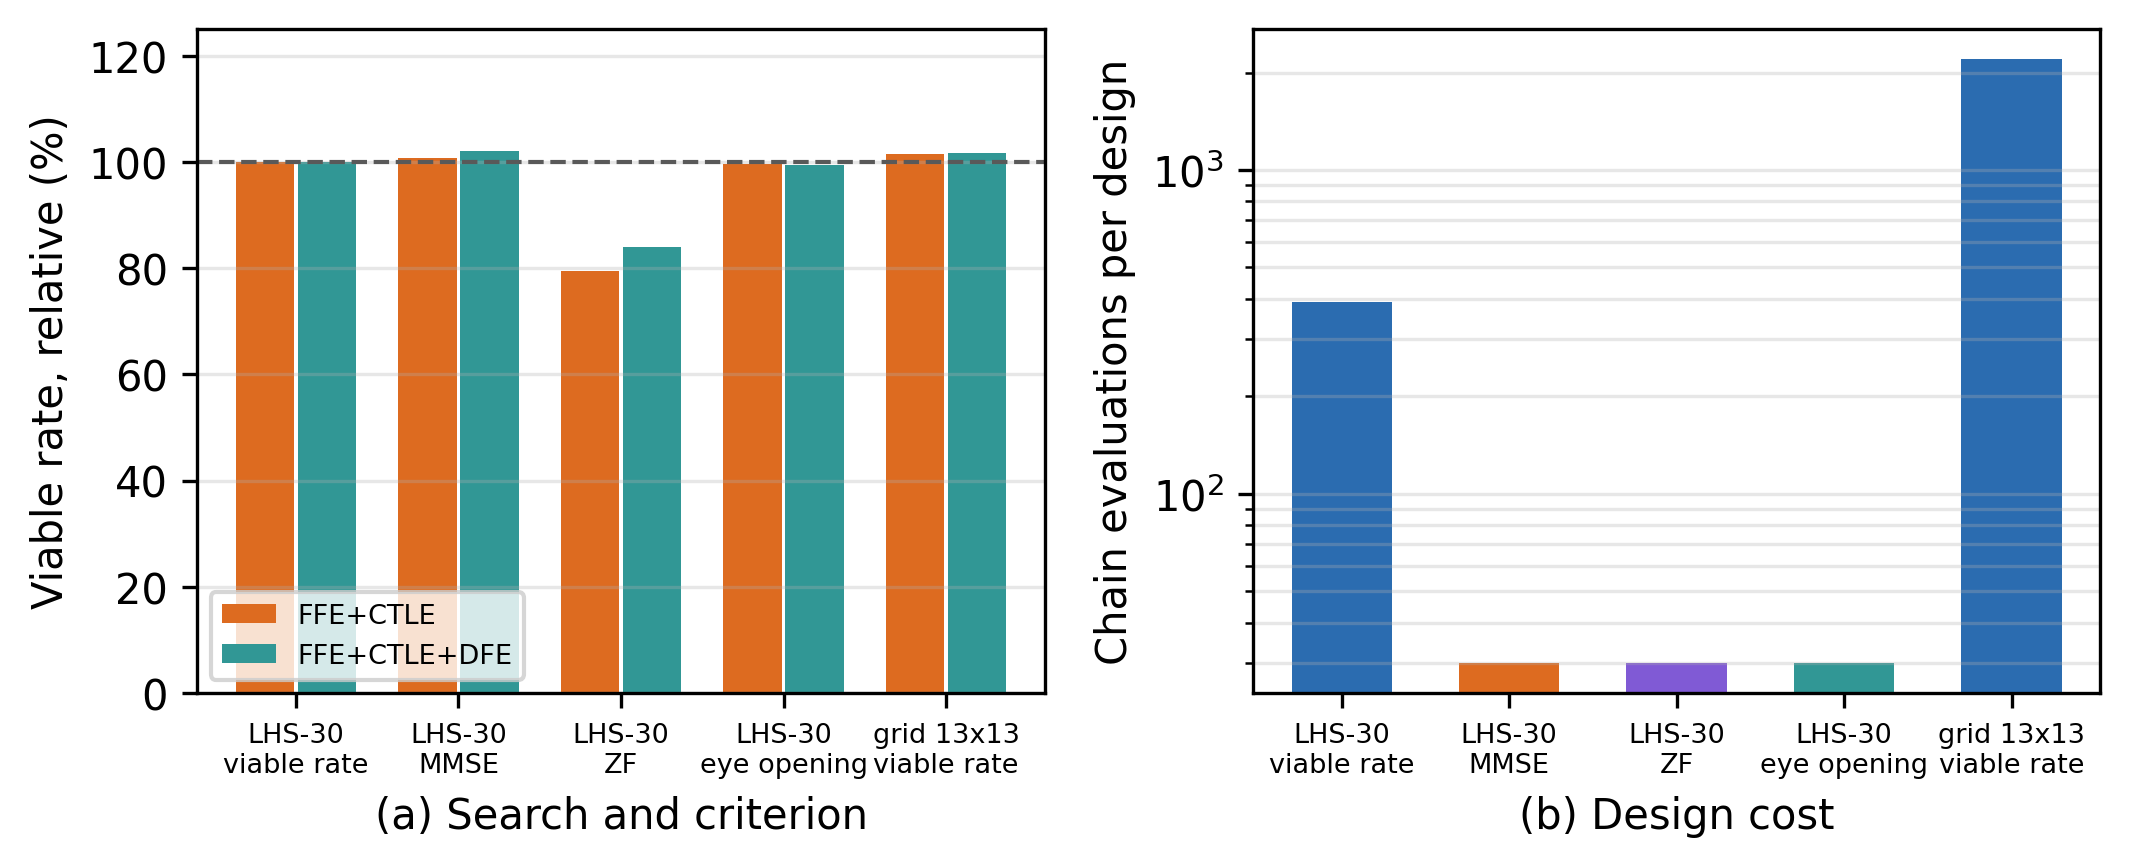
\includegraphics[width=\linewidth]{fig_baseline_criterios.png}
\caption{Standard tuning criteria against the procedure used in this work,
averaged over the FR-4 and Megtron~6 channels: (a)~viable rate relative to that
procedure, for the linear chain and for the chain with decision feedback, and
(b)~chain evaluations consumed by each design.}
\label{fig:baseline}\end{figure}

\subsection{Generality of the design rule}
\label{sec:generalidad}
A design rule derived with one equalizer and one objective is only useful if it
survives both. The re-DoE was therefore repeated over five channels spanning an
order of magnitude in bandwidth, for six configurations: the CTLE of this work
(A0), the same with wideband poles at $25/50$~GHz (A1) and with narrowband
poles at $8/16$~GHz (A2), a two-zero CTLE with zeros at $\omega_z$ and
$2\omega_z$ (A3), a higher DC gain $A_{DC}=4.0$ (A4), and A0 optimized for
worst-eye opening instead of viable rate (A5). Fitting
$f_z^{\ast}=k\,\mathrm{BW}^{p}$ per configuration gives the results of
Fig.~\ref{fig:generalidad}.

Two things must be separated. The \emph{direction} of the rule is general: $p$
is positive in all six configurations, so the optimal zero always migrates
upward as the channel widens, and a tuning derived on a narrow channel is
always too soft for a wider one. The \emph{magnitude} is not: $p$ ranges from
$0.30$ to $0.94$ (mean $0.71$). The two-zero architecture weakens the
dependence most ($p=0.30$, $R^2=0.42$), which is consistent with its second
zero supplying part of the high-frequency boost so that the first one need not
migrate as far, and the eye-opening objective is the noisiest fit
($R^2=0.73$)---the same weakness of the staged objective already seen in
Table~\ref{tab:r5}. The DC gain is irrelevant: A4 reproduces A0 exactly,
confirming that the optimal zero is set by the loss profile of the channel and
not by the flat gain of the equalizer. The rule therefore transfers as a
\emph{direction and a procedure}, not as a coefficient---which is the same
conclusion this work reaches for the tuning itself, now applied one level up:
the design rule must also be re-derived for a different equalizer architecture.

Making the rule quantitative also requires naming the bandwidth. The
conventional $-3$~dB corner does not order these channels the way their optimal
zeros are ordered: FR-4 under \textit{equal\_il} has a wider $-3$~dB bandwidth
than Megtron~6 under the same criterion ($0.59$ against $0.44$~GHz) yet a
\emph{lower} optimal zero ($2.35$ against $2.65$~GHz). The frequency at which
the channel has lost $10$~dB does order them consistently ($3.07$ against
$3.52$~GHz), and is the descriptor used above. This is physically reasonable:
the zero is placed where the equalizer must work, not where the channel first
begins to droop.

\begin{figure}[!t]\centering
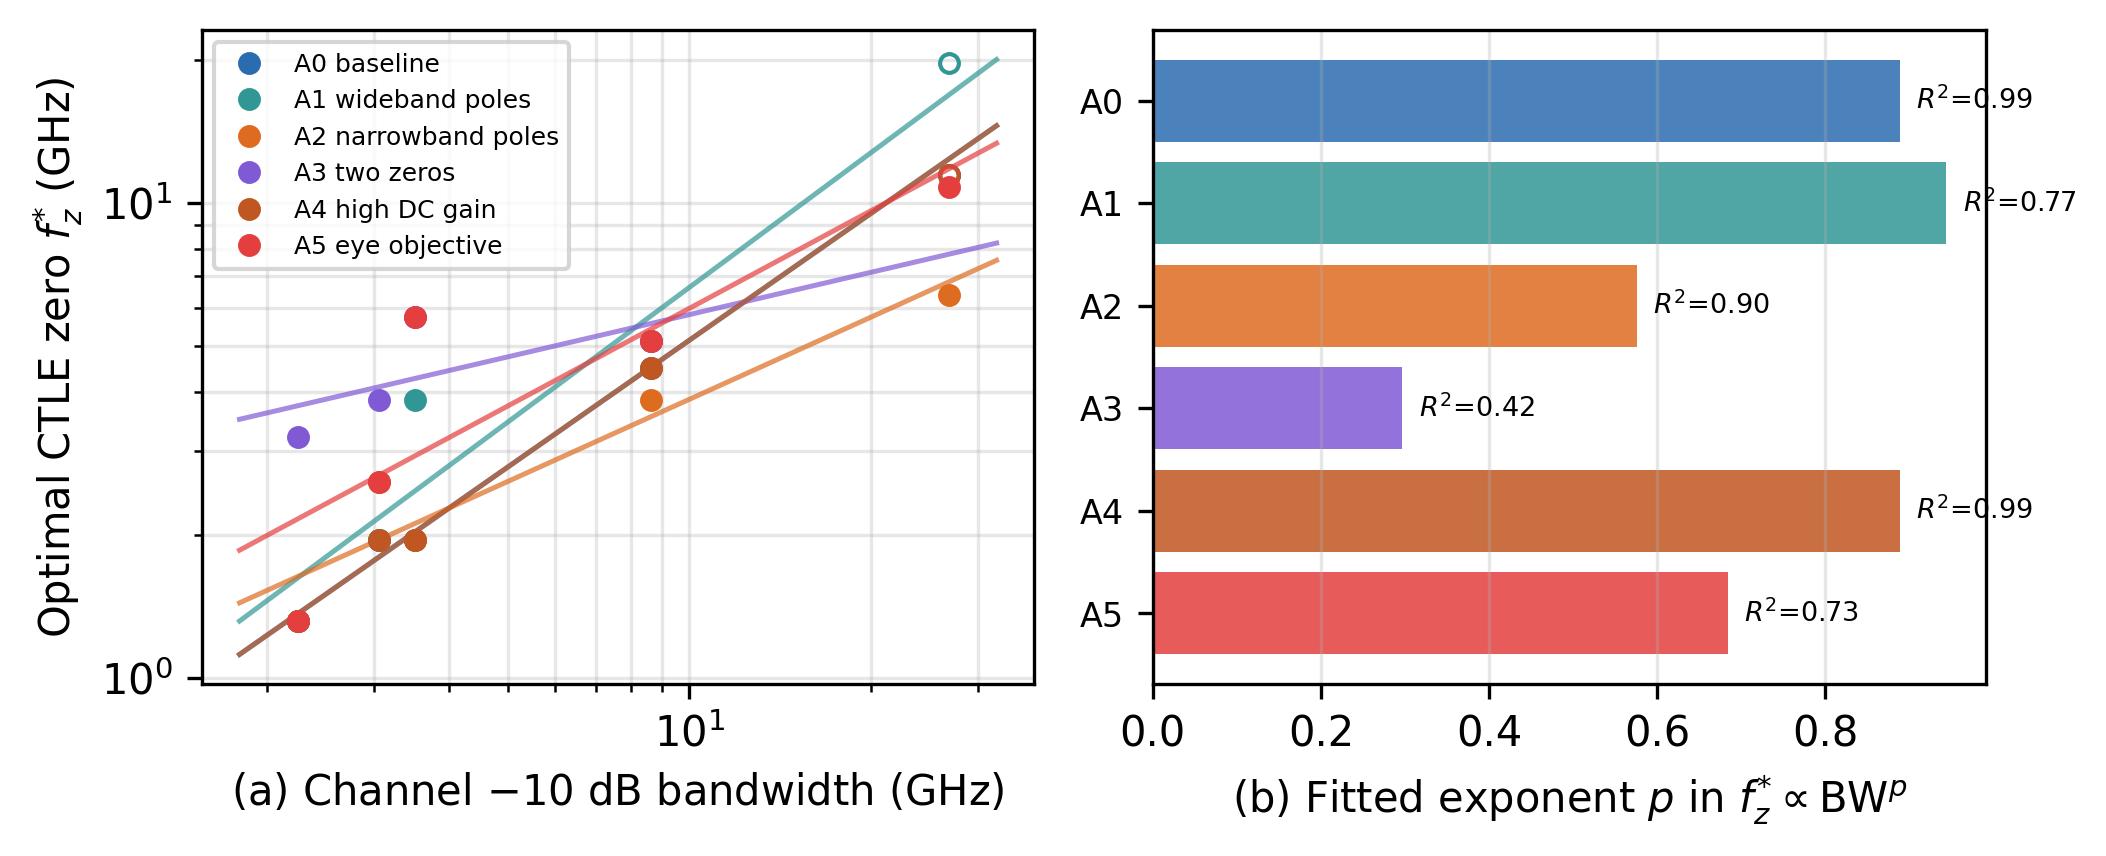
\includegraphics[width=\linewidth]{fig_generalizacion_wz.png}
\caption{Generality of the scaling rule across equalizer architectures and
optimization objectives: (a)~optimal CTLE zero against the channel $-10$~dB
bandwidth, with the fitted power law per configuration (open markers denote
channels whose objective saturates within the rate sweep, excluded from the
fit), and (b)~the fitted exponent $p$. A0 and A4 coincide exactly, so their
markers overlap.}
\label{fig:generalidad}\end{figure}

\subsection{Timing margin and robustness to jitter}
The horizontal margin was evaluated through the error-rate curve versus the
sampling phase. The horizontal opening reflects the same mismatch as the
vertical margin: the RC channel reaches $0.51$ of a unit interval after the
linear equalizer, against $0.18$ and $0.15$ on FR-4 and Megtron~6
(Fig.~\ref{fig:banera}). With the feedback equalizer in the loop, the
two-dimensional margin follows the vertical one and the choice of linear
equalizer does not alter the horizontal margin, in line with the
voltage--timing margin trade-off described for high-speed links
\cite{4509472}. The injection of random and deterministic jitter
(Fig.~\ref{fig:estres}) shows that, in the considered test bench, the viable
rate does not degrade appreciably up to a deterministic jitter on the order
of $0.2$ to $0.25$ of a unit interval, and that the closure level depends on
the assumed model: close to $0.35$ with a dual-Dirac worst-case
representation, and to $0.4$ with sinusoidal periodic jitter
\cite{805809,7202856,10584882,7571656}.

\begin{figure}[!t]\centering

\includegraphics[width=\linewidth]{fig_banera_escenarios.png}
\caption{Error rate versus sampling phase (horizontal eye opening) per
equalization stage on the FR-4 channel.}
\label{fig:banera}\end{figure}

\begin{figure}[!t]\centering

\includegraphics[width=\linewidth]{fig_estres_jitter.png}
\caption{Two-dimensional viable rate as a function of the injected
deterministic jitter, for the inherited and the co-optimized equalization.}
\label{fig:estres}\end{figure}

\subsection{Generalization: PAM-8 with the same equalization chain}
Applying the co-design to PAM-8 (eight levels in $\pm3$~V) without
re-optimization, the BER ordering among no equalization, FFE+CTLE and
FFE+CTLE+DFE is preserved (Fig.~\ref{fig:pam8ber}). The viable gross
throughput of PAM-8 does not
exceed that of PAM-4: they coincide with FFE+CTLE and PAM-4 exceeds it
without equalization and with FFE+CTLE+DFE
(Tables~\ref{tab:r4a}--\ref{tab:r4b}, Fig.~\ref{fig:throughput}). The rates
in this comparison come from an independent PAM-4/PAM-8 sweep on a
$1\,\mathrm{GBaud}$ grid under identical channel and co-design, so the PAM-4
values ($2,9,14$~GBaud) differ from Table~\ref{tab:r1}
($2.88,9.76,13.73$~GBaud) because of the sweep granularity (no
interpolation); the PAM-4 versus PAM-8 comparison is valid because both
share the same grid.

\begin{table}[!t]
\caption{Viable Rate (GBaud, $\mathrm{BER}\le10^{-2}$; Sweep on a 1~GBaud
Grid, no Interpolation).}
\label{tab:r4a}\centering
\begin{tabular}{lcc}
\hline
\textbf{Configuration} & \textbf{PAM-4} & \textbf{PAM-8} \\
\hline
No equalization & 2 & 1 \\
FFE + CTLE & 9 & 6 \\
FFE + CTLE + DFE & 14 & 8 \\
\hline
\end{tabular}
\end{table}

\begin{table}[!t]
\caption{Viable Gross Throughput (Gb/s) $=$ Viable Rate $\times$ Bits per
Symbol, Without Discounting FEC Overhead.}
\label{tab:r4b}\centering
\begin{tabular}{lcc}
\hline
\textbf{Configuration} & \textbf{PAM-4} & \textbf{PAM-8} \\
\hline
No equalization & 4 & 3 \\
FFE + CTLE & 18 & 18 \\
FFE + CTLE + DFE & 28 & 24 \\
\hline
\end{tabular}
\end{table}

\begin{figure}[!t]\centering

\includegraphics[width=\linewidth]{fig_pam8_ber.png}
\caption{Semi-analytical BER versus symbol rate for PAM-8, in the three
equalization configurations.}
\label{fig:pam8ber}\end{figure}

\begin{figure}[!t]\centering

\includegraphics[width=\linewidth]{fig_throughput.png}
\caption{Viable gross throughput (Gb/s) per equalization configuration,
PAM-4 against PAM-8.}
\label{fig:throughput}\end{figure}

%% =====================================================================
\section{Discussion}
\label{sec:discussion}

The results support a more specific hypothesis than simply stating that
equalization helps: the co-design must be matched to the channel and to the
full receiver objective. On the RC benchmark, the FFE+CTLE linear
equalization and the subsequent addition of the DFE successively raise the
viable rate above the intrinsic channel limit. The magnitude of the increase
depends on the adopted reference---the theoretical limit at which the Nyquist
frequency equals the bandwidth, or the viable rate measured without
equalization---so it is best interpreted as a multiplicative factor rather
than as a single figure. That the ladder approximation reproduces the
reference result supports the validity of the simulator and confirms that
the sweep measures the intended phenomenon and not a numerical artifact.

The extension to physics-based dispersive channel models qualifies the role of the RC
model. At equal insertion loss at the Nyquist frequency, the channels with
frequency-dependent losses tolerate, without equalization, a higher rate
than the RC channel, whose diffusive response presents a more prolonged ISI
tail \cite{8861405}; the RC model therefore tends to overestimate the link
difficulty at equal loss. Moreover, the co-design optimized on the RC
channel does not transfer without adjustment to the dispersive channel model: the
optimal CTLE zero increases with the channel bandwidth, so re-optimizing the
equalization per substrate recovers viable rate, more appreciably on short
low-loss lines \cite{11169790}. This dependence is consistent with the loss
variation between laminates \cite{9785524,10385078,915226}. On low-loss
channels, linear equalization can even reduce the viable rate by amplifying
noise unnecessarily, which confirms that its usefulness is tied to the
channel severity.

The Megtron~6 fixed-length case deserves specific analysis for its striking
figures (without equalization, $40$~GBaud; with decision feedback, above
$60$). At $10$~inches, this low-loss-tangent laminate ($\tan\delta=0.004$)
presents an insertion loss of barely $2$~dB at the Nyquist frequency, so the
channel hardly limits the signaling in the band of interest: the factor that
bounds performance is not the channel ISI but the receiver---the
input-referred noise and the finite bandwidth. In that regime, the CTLE
boost amplifies noise without appreciable ISI to compensate, so linear
equalization \emph{reduces} the viable rate (over-equalization); the decision
feedback, which cancels ISI without amplifying noise, does not suffer that
penalty and extends the rate up to the limit imposed by the receiver noise.
Far from being anomalous, this behavior illustrates the central message of
the work: the usefulness---and even the sign---of each equalization stage's
benefit depends on the channel severity, so equalization must be sized on the
specific channel model. It is worth noting that rates of several tens of
GBaud in PAM-4 exceed the nominal operating point and must be interpreted as
a limit of the test bench---which does not incorporate reflections, vias or
crosstalk---and not as a deployment proposal.

The examination of the operating point qualifies this reading. At the
nominal rate, the transmit FFE alone already opens the eye, so there the CTLE
and DFE add margin, not viability; their value becomes apparent when
extending the rate, where the eye opening and the BER degrade abruptly. This
contrast warns that evaluating equalization at a single point can
misrepresent its role, and justifies adopting the rate reach as the primary
indicator. The addition of the DFE further illustrates that equalization is
not free: with the eye already open, the decision feedback adds little and
can slightly reduce the margin, consistent with the erroneous-decision and
error-propagation effects described for the DFE \cite{10584882,9505189}. Its
net benefit is therefore concentrated in the severe-channel regime.

The PAM-8 stress case offers two observations. First, the performance
ordering between configurations is preserved when migrating to a denser
constellation, which indicates that the co-design---oriented to compensating
the channel and not the constellation---generalizes. Second, under a fixed
amplitude budget, the additional bits per symbol of PAM-8 do not translate
into higher viable gross throughput: its smaller reach offsets the gain in
bits and equals PAM-4 only with the full equalization chain. This behavior is
consistent with the margin penalty inherent to higher modulation orders in
bandwidth-limited systems \cite{8963973} and with the motivation for PAM-4 as
a compromise between spectral density and robustness \cite{7964959}; it
suggests that, on this channel, increasing the baud rate dominates over
increasing the modulation order.

Beyond the vertical amplitude margin, the horizontal timing margin was
examined by building the error-rate curve versus the sampling phase and
injecting random and deterministic jitter. With the decision-feedback
equalizer in the loop, the two-dimensional margin follows the vertical one:
in the considered test bench, the viable rate does not degrade appreciably up
to a deterministic jitter on the order of $0.2$ to $0.25$ of a unit interval,
so for jitter budgets in that range the timing does not limit the obtained
reach \cite{7202856,10584882}. This voltage--timing margin trade-off is
consistent with the statistical margin simulation frameworks for high-speed
links \cite{4509472}. The jitter level that closes the link depends on the
assumed model---a dual-Dirac worst-case representation places it near $0.35$
of a unit interval, while a sinusoidal periodic jitter shifts it toward $0.4$
with a more gradual degradation \cite{805809,7571656}---but in all cases the
choice of linear equalizer does not alter the horizontal margin, since the
decision feedback cancels the tail interference at each sampling instant.

The joint co-design of the linear and feedback stages, formalized as the
design rule of Section~\ref{sec:results}, follows from this evidence:
maximizing the linear eye in isolation amplifies noise that the feedback
stage would otherwise have avoided, whereas optimizing both jointly yields a
softer linear equalizer that delegates the tail cancellation to the decision
feedback \cite{11169790,11346689}.

The scope of these results is bounded by several simplifications. The
dispersive line model incorporates skin effect and dielectric loss; the
surface roughness was treated through a first-order correction and a
sensitivity analysis bounded its effect (second order against dielectric loss
and length). Reflections are treated as a bounded case rather than a full
model: Section~\ref{sec:reflexiones} quantifies a single midpoint
discontinuity, but multiple interacting discontinuities, crosstalk and modal
dispersion are not modeled, and a rigorous validation would require
correlation with measured $S$-parameters or full-wave solvers
\cite{9134991,5089870}. As an
intermediate step in that direction, the chain was contrasted against an
independent circuit simulator: it agrees in the frequency response and, on
the RC channel, in the time-domain eye diagram, which indicates that the
figures do not depend on the particular implementation; the time-domain
representation of the dispersive channel in that simulator is limited by the
non-rational nature of the skin-effect loss, so its eye is evaluated in the
frequency domain. The DFE is fitted with the transmitted sequence, so its
figures represent a performance bound rather than a blind adaptive
implementation. The ladder approximation reproduces the RC line with a finite
order, somewhat conservative in the band that equalization exploits relative
to the analytical transfer function. The BER is a semi-analytical estimate
under a Gaussian assumption, suitable for avoiding the cost of Monte Carlo
counting of low error rates \cite{6248821}; it was validated against direct
counting in the region near the pre-FEC threshold, where both agree and the
estimator is slightly conservative, although it does not replace a
characterization of non-Gaussian tails at very low error rates; in that sense
it is consistent with the statistical-eye methods in the literature
\cite{7202856,10415105}. Finally, the co-design was explored in a
two-variable subspace through Latin hypercube sampling, amenable to extension
with sequential or Bayesian-optimization schemes \cite{11309336}, and the eye
was evaluated at a single operating point.

The most consequential of these limitations is that the study is entirely
simulated, and it is worth stating plainly what that does and does not permit.
An experimental validation is feasible with standard laboratory equipment and
would require a test coupon carrying FR-4 and low-loss traces of the modeled
lengths with well-characterized launches, vector network analyzer
$S$-parameters over at least twice the highest Nyquist frequency examined
here, a PAM-4 pattern source with hardware error counting, and a transceiver
whose FFE, CTLE and DFE settings can be programmed to the tunings reported
above. What such a measurement would settle is the absolute rates, which
depend on parts of the link deliberately left out---packages, connectors,
crosstalk, and a DFE adapting blind rather than from the known sequence---and
whether the RLGC model reproduces the measured loss and delay of real
laminates. What it would be less likely to overturn is the relative
comparisons that constitute the results of this work, since each is computed
between configurations evaluated on the same bench and under the same receiver
model; that expectation is an argument, however, not a proof. Simulation-only
evidence is therefore not offered here as equivalent to measurement: the
cross-checks against the analytical response, the exported $S$-parameters and
an independent circuit simulator verify that the chain is implemented as
described, which is a weaker claim than verifying that it matches a physical
board.

%% =====================================================================
\section{Conclusion}
\label{sec:conclusion}

This work quantified, under a single reproducible and cross-validated test
bench, how far an equalizer co-design optimized on an idealized RC channel
transfers to physical dispersive channels, and how the sign of each
equalization stage's benefit depends on the channel severity once the
receiver noise is referred to the input.

The ladder approximation reproduces the analytical transfer function of the
RC channel and, on it, the reference result, which validates the simulator;
a cross-check in an independent circuit simulator, which reproduces the
frequency response of the chain and its eye diagram over the RC channel,
reinforces this validation. Replacing the RC model with a transmission line
with frequency-dependent losses confirms that the physics-based channel model is
dispersive, with an attenuation that grows with frequency and a propagation
delay absent from the diffusive model.

The central finding is that the co-design optimized on the RC channel does
not transfer without adjustment to the dispersive channel model: the optimal zero of
the linear equalizer increases with the channel bandwidth, and re-optimizing
the equalization per substrate increases the FFE+CTLE viable rate by up to
$72\%$ (FR-4) and $96\%$ (Megtron~6), more appreciably on short low-loss
lines. On
those benign channels, a linear equalization that is too aggressive can even
reduce the viable rate by amplifying noise; jointly co-optimizing the linear
boost and the decision feedback, taking the full chain as the objective,
avoids this penalty (exceeding staged tuning by up to $12.4\%$) and leads to
a softer boost that delegates the tail cancellation to the feedback. The
timing margin, evaluated under random and deterministic jitter, is robust:
with the decision feedback in the loop, the horizontal margin follows the
vertical one and does not degrade appreciably for deterministic jitter up to
the order of one fifth of a unit interval. In the PAM-8 stress case, the
configuration ranking is preserved, but under a fixed amplitude budget PAM-8
does not increase the viable gross throughput relative to PAM-4.

Overall, the results show that equalization co-design must be sized to the
dispersive channel model and evaluated under the full receiver objective to avoid
overstating, or even reversing, its benefit. The reported gain is attributable
to the equalization---and not to optimistic receiver assumptions---because it
was evaluated with input-referred noise and finite bandwidth. The study shows
that the co-design must be carried out on the physics-based channel model and not on its
idealization. As future work, it is suggested to refine the jitter model
toward more realistic distributions, to validate the dispersive model against
measured scattering parameters or full-wave solvers, to adopt standard
channel-operating-margin and statistical error-rate-estimation metrics, and
to validate the link experimentally on a physical trace with hardware error
counting.

%% =====================================================================
\bmsubsection*{Data Availability Statement}
The complete reproducibility package supporting this study is openly
available on GitHub at
\url{https://github.com/sefran1020/equ-max-band_high-speed} (release commit
\texttt{5d8784c}), released under the MIT License. The package is
self-contained and traceable: it provides the frequency-domain simulation
chain, the LTspice cross-validation netlists and subcircuits, the exported
Touchstone $S$-parameters, the intermediate \texttt{CSV} datasets, and a
traceability matrix that maps every figure and table in this article to the
script and data that generate it. The verified environment is Python~3.14
(NumPy, SciPy, Matplotlib) and LTspice ADI~26.0.2.1. An archival snapshot
with a persistent Zenodo DOI will be deposited upon acceptance.

\bmsubsection*{Declaration of Generative AI and AI-Assisted Technologies}
During the preparation of this work, the authors used Claude Code and
Antigravity CLI in order to organize information, assist with data analysis,
structure the repository, and improve the drafting of the manuscript. After
using these tools, the authors reviewed and edited the content as needed and
take full responsibility for the content and results of the published
article.

\bmsubsection*{Acknowledgments}
The authors thank the Universidad Nacional Pedro Ruiz Gallo for institutional
support.

%% =====================================================================
\bibliographystyle{IEEEtran}
\bibliography{references}



% Legacy IEEE author biographies are intentionally excluded from the Wiley
% submission. They are retained below only as source-history comments and are
% not part of the compiled manuscript.
\iffalse

\begin{IEEEbiography}[{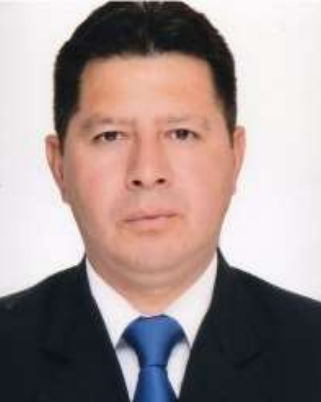
\includegraphics[width=1in,height=1.25in,clip,keepaspectratio]{autores/francisco.png}}]{Segundo F. Segura-Altamirano}
	He received a bachelor's degree in Electronic Engineering from the National University of San Marcos in Lima, Peru, in 1996. He completed his master's studies in Telecommunications and Networking at the Technological University of Peru, Lima, in 2021, and obtained another master's degree in Applied Mathematics from the National University Pedro Ruiz Gallo, Lambayeque, Peru.
	
	From 1996 to 2003, he worked as a Technical Manager for telecommunications operators, carrying out activities related to the operation and maintenance of broadband optical networks. In 2004, he joined as an Assistant Professor in the Department of Electronic Engineering at the National University Pedro Ruiz Gallo. Currently, he is an Associate Professor in the areas of telecommunications, broadband networks, image processing, and machine learning.
	
	He is the author of articles on image processing, broadband networks, and machine learning.
	
\end{IEEEbiography}


\begin{IEEEbiography}[{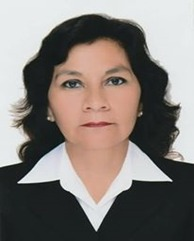
\includegraphics[width=1in,height=1.25in,clip,keepaspectratio]{autores/dianaM.jpeg}}]{Diana M. Castro-C\'ardenas} Ph.D., is a Principal Lecturer in the Department of Mathematics at the Faculty of Physical Sciences and Mathematics, National University Pedro Ruiz Gallo. She earned her Bachelor's degree in Mathematics from the National University San Luis Gonzaga de Ica in 1993, followed by a Master's degree in Applied Mathematics from the National University Pedro Ruiz Gallo in 2016, and a Doctorate in Education from the University Cesar Vallejo in 2020. Her research interests encompass flipped classrooms, neural networks, finite elements, numerical methods, and optimization.
	
\end{IEEEbiography}

\begin{IEEEbiography}[{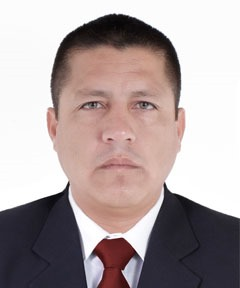
\includegraphics[width=1in,height=1.25in,clip,keepaspectratio]{autores/carlos02.jpeg}}]{Carlos L. Oblitas-Vera}
received the Eng. degree in electronic engineering from the Universidad Privada Antenor Orrego, Trujillo, Peru, the M.S. degree in artificial intelligence from the Universidad Internacional de La Rioja, Mexico, the M.S. degree in education, with a specialization in teaching and educational management, from the Universidad César Vallejo, Peru, and the Ph.D. degree in mechanical and electrical engineering sciences from the Universidad Nacional Pedro Ruiz Gallo, Lambayeque, Peru. He has also completed specialized studies in electronic sciences with an emphasis on biomedical engineering.

His professional experience includes working as a resident engineer in various hospitals throughout Peru, specializing in the maintenance of biomedical equipment, X-ray systems, and clinical laboratory equipment. Since 2003, he has been an Associate Professor with the Department of Electronic Engineering, Universidad Nacional Pedro Ruiz Gallo. His research interests include automation, biomedical engineering, artificial intelligence, and energy optimization.
	
	
\end{IEEEbiography}


\begin{IEEEbiography}[{
\includegraphics[width=1in,height=1.25in,clip,keepaspectratio]{autores/alcides.png}}]{Alcides Ra\'ul Cuti Guti\'errez}
	received the B.S. degree in mathematics and the Ph.D. degree in educational sciences from the National University Pedro Ruiz Gallo (UNPRG), Lambayeque, Peru, and the M.S. degree in education, with a specialization in teaching and educational management, from César Vallejo University, Trujillo, Peru.
	
	Since 1999, he has been an Associate Professor with the Department of Mathematics, National University Pedro Ruiz Gallo. He serves as an advisor and thesis director for pure and applied mathematics at both the undergraduate and graduate levels. He is a specialist in mathematical logic (PRONAFCAP) and the author of the book Differential Calculus and its Applications. His academic experience includes teaching positions at several Peruvian institutions, including San Pedro University (Cajamarca), the University of Chiclayo (UDCH), the Central University of Venezuela (UCV branches in Chiclayo and Trujillo), and the National Pedagogical University (UPN, Lima). He is also a specialist in pedagogical research with the ELIM Institute, Chiclayo.
	
	
\end{IEEEbiography}



\begin{IEEEbiography}[{
\includegraphics[width=1in,height=1.25in,clip,keepaspectratio]{autores/janet}}]{Janet R. Aquino-Lalupu}
	received the B.S. degree in Computer and Systems Engineering from Universidad Privada Antenor Orrego, Peru, and the M.B.A. degree with a concentration in Business Management from Universidad Nacional Pedro Ruiz Gallo, Peru, where she also completed her doctoral studies in Education. She is certified as a Level IV Researcher by RENACYT.
	
	She has 29 years of experience in academia and is currently a Professor and Researcher with the Universidad Nacional Pedro Ruiz Gallo, and a Professor with the Universidad Tecnológica del Perú. She has an extensive track record in professional training and leading research projects. Her research interests include digital transformation, artificial intelligence, business intelligence, and technologies applied to education. Her professional commitment focuses on promoting innovation and contributing to scientific and technological development through research and human talent cultivation.
\end{IEEEbiography}



\begin{IEEEbiography}[{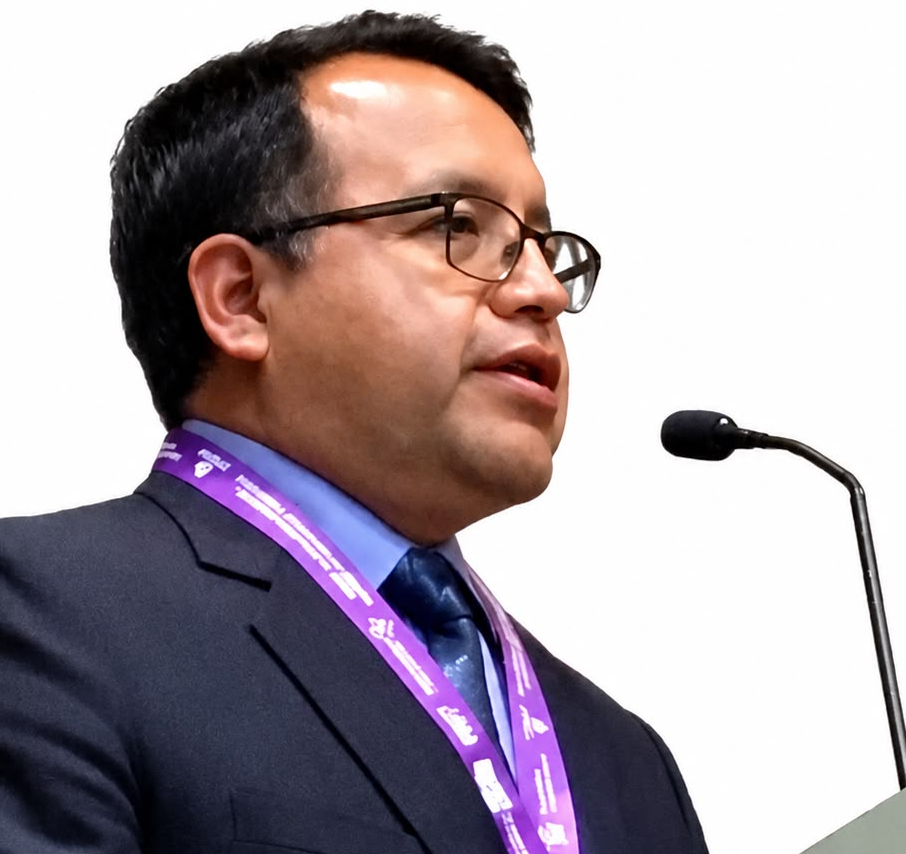
\includegraphics[width=1in,height=1.25in,clip,keepaspectratio]{autores/nilton}}]{Nilton C. German-Reyes}
	was born in Otuzco, La Libertad, Peru. He received the B.S. degree in Computer and Systems Engineering from Universidad Privada Antenor Orrego, Trujillo, Peru, and the M.B.A. degree with a concentration in Business Management from Universidad Nacional Pedro Ruiz Gallo, Lambayeque, Peru. He pursued doctoral studies in Sciences at Universidad Nacional Federico Villarreal, Lima, Peru, and received the Ph.D. degree in Education.
	
	He is currently a Full-Time Principal Professor with the Universidad Nacional Pedro Ruiz Gallo, Lambayeque, Peru. He is also certified as a registered researcher by RENACYT. His research interests include digital transformation, software engineering, computer science, software quality, machine learning, and artificial intelligence.
\end{IEEEbiography}
\fi

\end{document}
